\documentclass[twocolumn]{aastex63}

\usepackage{amsmath}
\usepackage{empheq}
\usepackage{mathrsfs}
\usepackage{textcomp}
%\usepackage{enumitem}   
\usepackage{gensymb}
\usepackage{hyperref}
\usepackage{graphicx}
\usepackage[caption=false]{subfig}
\usepackage{multirow}
\usepackage{longtable}
\usepackage{booktabs} % To thicken table lines
\usepackage{CJK}
\bibliographystyle{aasjournal}
\hypersetup{colorlinks, linkcolor={blue}, citecolor={blue}, urlcolor={blue}} 

%\usepackage{lineno}
% \linenumbers

\newcommand{\vdag}{(v)^\dagger}
\newcommand\aastex{AAS\TeX}
\newcommand\latex{La\TeX}

%%%%%%%%%%%%%%%%%%%%%%%%%%%%%%%%%%%%%%%%%%%%%%%%%%%%%%%%%%%%%%%%%%%%%%%%%%%%%%%%
%%
%% The following section defines new commands for comments from co-authors
%%
\definecolor{DarkOrange}{RGB}{204, 85, 0}
\definecolor{LincolnGreen}{RGB}{17, 102, 0}
\def\ion#1#2{#1$\;${\footnotesize\rm{#2}}\relax}

\newcommand{\yy}[1]{{\color{red} yy: {#1}}}
\newcommand{\kde}[1]{{\color{DarkOrange} kde: {#1}}}
\newcommand{\todo}[1]{{\color{magenta} to-do: {#1}}}

\newcommand{\rztf}{$r_\mathrm{ZTF}$}
\newcommand{\gztf}{$g_\mathrm{ZTF}$}
\newcommand{\tfl}{$t_\mathrm{fl}$}
\newcommand{\trise}{$t_\mathrm{rise}$}
\newcommand{\tbmax}{$t_{B,\mathrm{max}}$}
\newcommand{\package}[1]{\textsc{#1}}
%%
%%%%%%%%%%%%%%%%%%%%%%%%%%%%%%%%%%%%%%%%%%%%%%%%%%%%%%%%%%%%%%%%%%%%%%%%%%%%%%%%

%% Reintroduced the \received and \accepted commands from AASTeX v5.2
%\received{\today}
% \revised{January 10, 2019}
% \accepted{\today}
%% Command to document which AAS Journal the manuscript was submitted to.
%% Adds "Submitted to " the argument.

%\submitjournal{ApJ}

%%%%%%%%%%%%%%%%%%%%%%%%%%%%%%%%%%%%%%%%%%%%%%%%%%%%%%%%%%%%%%%%%%%%%%%%%%%%%%%%
%%
%% The following section outlines numerous optional output that
%% can be displayed in the front matter or as running meta-data.
%%
%% If you wish, you may supply running head information, although
%% this information may be modified by the editorial offices.
\shorttitle{AT2019dge: an Ultra-Stripped Envelope SN}
\shortauthors{Yao et al.}

%%
%% You can add a light gray and diagonal water-mark to the first page 
%% with this command:
\watermark{DRAFT}
%% where "text", e.g. DRAFT, is the text to appear.  If the text is 
%% long you can control the water-mark size with:
%% \setwatermarkfontsize{dimension}
%% where dimension is any recognized LaTeX dimension, e.g. pt, in, etc.
%%
%%%%%%%%%%%%%%%%%%%%%%%%%%%%%%%%%%%%%%%%%%%%%%%%%%%%%%%%%%%%%%%%%%%%%%%%%%%%%%%%

%% This is the end of the preamble.  Indicate the beginning of the
%% manuscript itself with \begin{document}.

\begin{document}
\pagenumbering{arabic}
\begin{CJK*}{UTF8}{gbsn}

\title{AT2019dge: a Fast-risng Type Ib Ultra-Stripped Envelope SN}

%\author[0000-0001-6747-8509]{Yuhan Yao (姚雨含)}\email{yyao@astro.caltech.edu}
%\affiliation{Cahill Center for Astrophysics, 
%             California Institute of Technology, 
%             1200 E.~California Boulevard, Pasadena, CA 91125, USA}

%\author{Friends}

% KDE, Mansi, Shri

% Zhihui


\begin{abstract}

We present observations of the hydrogen-deficient optical transient AT2019dge/ZTF18abfcmjw. With 
a rise to maximum light of $\lesssim 3$\,days over two magntiude in $g$ and $r$-bands, AT2019dge is 
the most rapidly-rising subluminous Type I supernova (SN) discovered so far. Spectra obtained shortly 
after discover reveal \ion{He}{II} flash emission, with broad \ion{He}{I} features developed $\sim12$\,d 
after peak luminosity. \todo{more to come.} AT2019dge poses chanllenge for existing models of 
fast-rising SNe.

\end{abstract}

%% Keywords should appear after the \end{abstract} command. 
%% See the online documentation for the full list of available subject
%% keywords and the rules for their use.
\keywords{supernovae: general -- supernovae: individual (AT2019dge/ZTF18abfcmjw) -- surveys}

%% From the front matter, we move on to the body of the paper.
%% Sections are demarcated by \section and \subsection, respectively.
%% Observe the use of the LaTeX \label
%% command after the \subsection to give a symbolic KEY to the
%% subsection for cross-referencing in a \ref command.
%% You can use LaTeX's \ref and \label commands to keep track of
%% cross-references to sections, equations, tables, and figures.
%% That way, if you change the order of any elements, LaTeX will
%% automatically renumber them.
%%
%% We recommend that authors also use the natbib \citep
%% and \citet commands to identify citations.  The citations are
%% tied to the reference list via symbolic KEYs. The KEY corresponds
%% to the KEY in the \bibitem in the reference list below. 

\vspace{1em}

\section{Introduction}
Type Ib/c supernovae (SNe Ib/c) are explosions of massive stars that lost their 
hydrogen envelopes. Their typical rise time ($t_{\rm rise}\approx 20\,{\rm d}$) and peak luminosity 
($M_{R\rm , peak} \approx -18$\,mag) suggest ejecta mass of $M_{\rm ej}\approx 2\, M_\odot$ and 
$^{56}$Ni mass 
of $M_{\rm Ni}\approx 0.2\, M_\odot$ \citep{Drout2011, Prentice2019}. Today, a growing number of 
subluminous and rapidly-evolving SNe Ib/c are discovered by wide-field optical surveys, such as 
SN2005ek \citep{Drout2013}, SN2010X \citep{Kasliwal2010}, iPTF14gqr \citep{De2018}, and the class of 
Ca-rich gap transients \citep{Kasliwal2012}. However, the physical origin of this population of SNe still 
remains largely elusive. 

Theoretical interpretation for faint and fast SNe include scenarios not related to the explosion of 
massive stars \citep{Shen2010, Sim2012, Metzger2009, Margalit2016}, an ultra-stripped massive star 
progenitor \citep{Tauris2015}, core-collapse supernovae (CCSNe) with fallback \citep{Moriya2010}, and
explosions of extended helium giant stars \citep{KleiserFuller2018}. Interaction with circumstellar 
material (CSM) and alternative power sources, on the other hand, are always invoked to explain 
more brighter and slow-evolving events (e.g. \citealt{Chevalier2011, Hotokezaka2017}).

Here we report observations of the rapidly rising ($t_{\rm rise}\lesssim3$\,d) subluminous ($M_{R\rm , 
peak} \approx -16$\,mag) helium-rich event AT2019dge discovered by the Zwicky Transient Facility 
(ZTF; \citealt{Bellm2019b};  \citealt{Graham2019}), and put it in the context of ultra-stripped envelope 
SNe. Calculations in this paper assume a $\Lambda$CDM cosmology with $H_0= 70 \, \rm km \, s^{-1}\, 
Mpc^{-1}$, $\Omega_m = 0.27$ and $\Omega_{\Lambda} = 0.73$ \citep{Komatsu2011}. UT times are 
used throughout the paper. Alongside this paper, we have released our open-source analysis and all of 
the data utilized in this study at \url{https://github.com/yaoyuhan/AT2019dge}. All spectra and 
photometry will also be made available by the WISeREP repository \citep{Yaron2012}.

\section{Observations} 
\subsection{The Detection and SN Location}
\begin{figure}[htbp!]
    \centering
    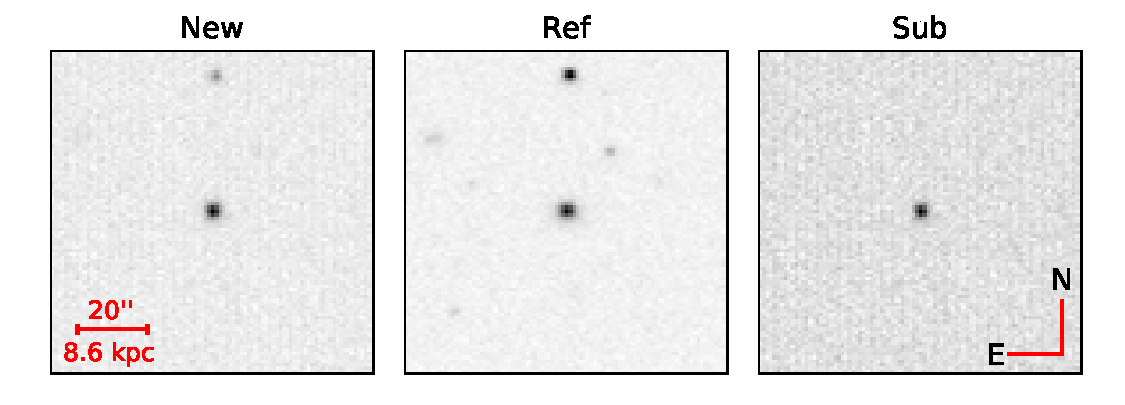
\includegraphics[width=\columnwidth]{figures/detection.pdf}
    \caption{ZTF $g$ band images centered on AT2019dge on Apr 10. From left to right are the new 
    image, the reference image, and the subtraction image. \ \label{fig:detection}}
\end{figure}
\begin{figure}
	\centering
	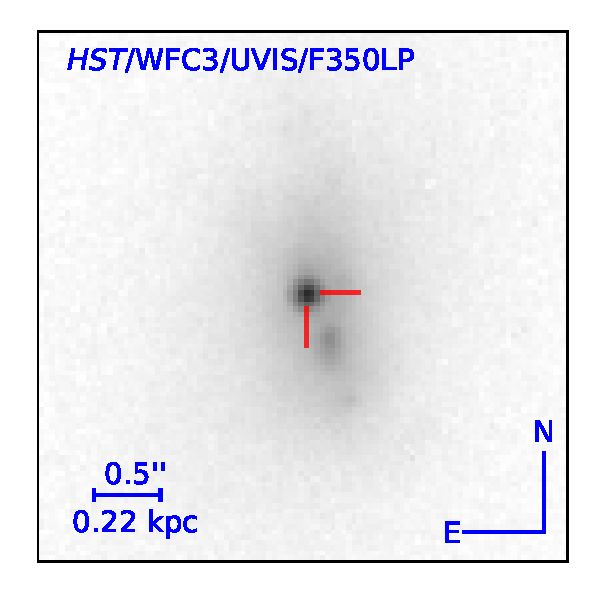
\includegraphics[width=0.6\columnwidth]{figures/offset.pdf}
	\caption{The position of AT2019dge (red crosshairs) in its host galaxy.
		%Images are combined using the prescription in \citet{Lupton2004}.
		\label{fig:offset}}
\end{figure}
\begin{figure*}[htbp!]
	\centering
	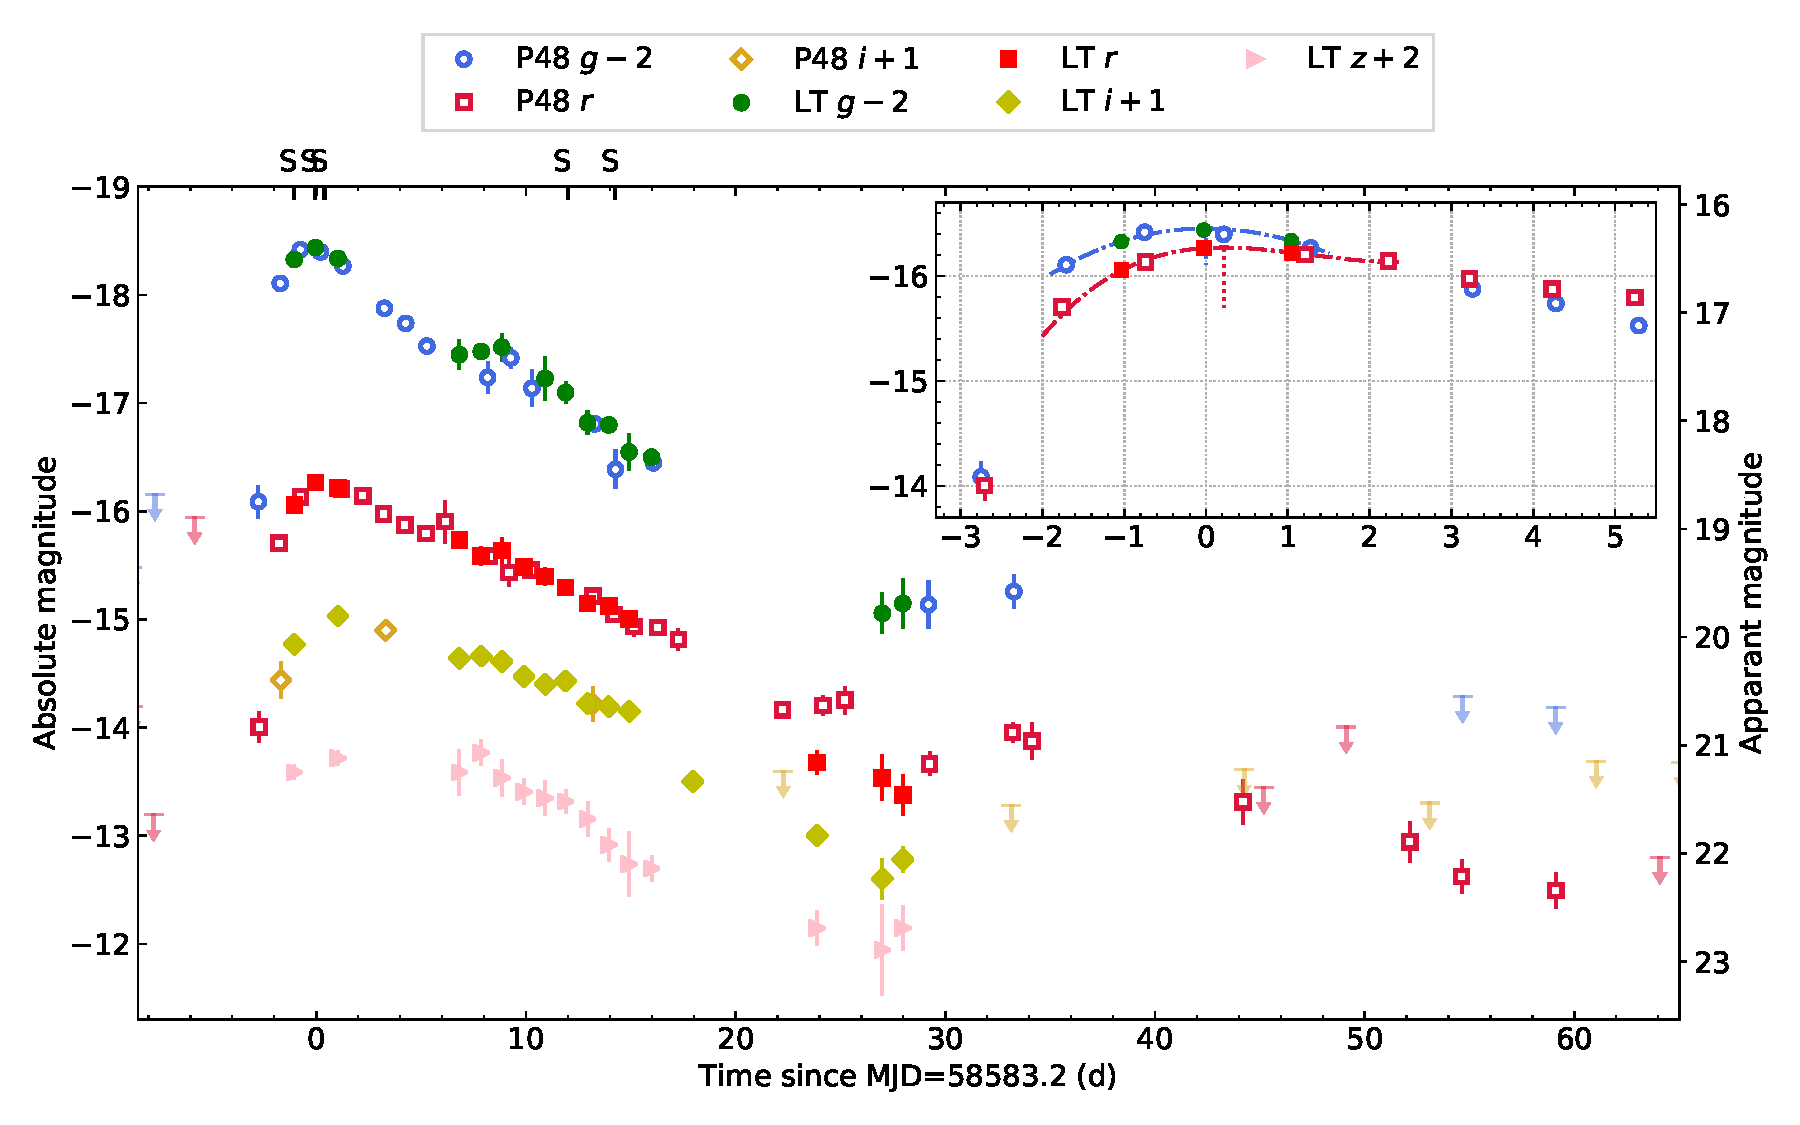
\includegraphics[width=\textwidth]{figures/lightcurve.pdf}
	\caption{Galactic extinction corrected light curve of AT2019dge. The inset shows 
		the light curve zoomed around the region of maximum light. Epochs of spectroscopy are marked 
		with the letter `S' along the upper axis.\label{fig:lightcurve}}
\end{figure*}
% In this section, I report values on Marshal
AT2019dge was first detected by ZTF using the Palomar Oschin Schmidt 48 inch (P48) telescope. On 
2019 April 7 10:18:46 (JD $=2458580.9297$), a $g$-band detection at 
$20.66\pm0.34$ mag and J2000 coordinates $\alpha = 
17^{\mathrm{h}}36^{\mathrm{m}}46.75^{\mathrm{s}}$, $\delta = 
+50^{\mathrm{d}}32^{\mathrm{m}}52.2^{\mathrm{s}}$
%$\alpha = 17^{\mathrm{h}}36^{\mathrm{m}}46.76^{\mathrm{s}}$, $\delta = 
%+50^{\mathrm{d}}32^{\mathrm{m}}52.5^{\mathrm{s}}$ (J2000) 
met the machine-learning thresholds \citep{Mahabal2019} and real-time alerts were generated 
\citep{Patterson2019}. On April 8, the transient was flagged by a science program filter on the 
GROWTH Marshal \citep{Kasliwal2019} that is designed to look for fast evolving transients. 
Figure~\ref{fig:detection} shows the ZTF detection image on April 10. AT2019dge resildes in a compact 
galaxy SDSS J173646.73+503252.3 at the redshift of $z=0.0213$ (See Appendix 
\ref{subsec:appspec_data}). Since AT2019dge is offset from the nucleus of the host in the 
\textit{Hubble Space Telescope} ($HST$) image (Figure~\ref{fig:offset}), the explosion can not be a 
tidal distruption event.

\begin{figure*}[htbp!]
	%
	\centering
	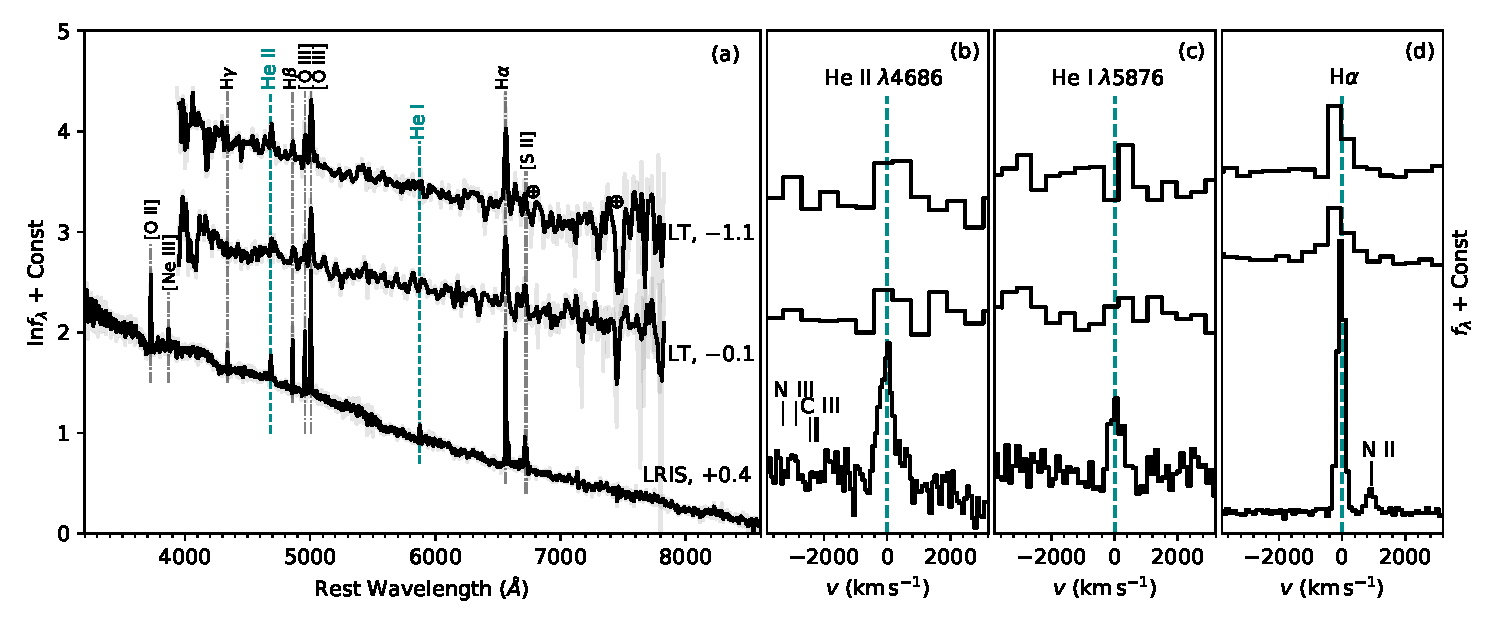
\includegraphics[width=\textwidth]{figures/spectra_early.pdf}
	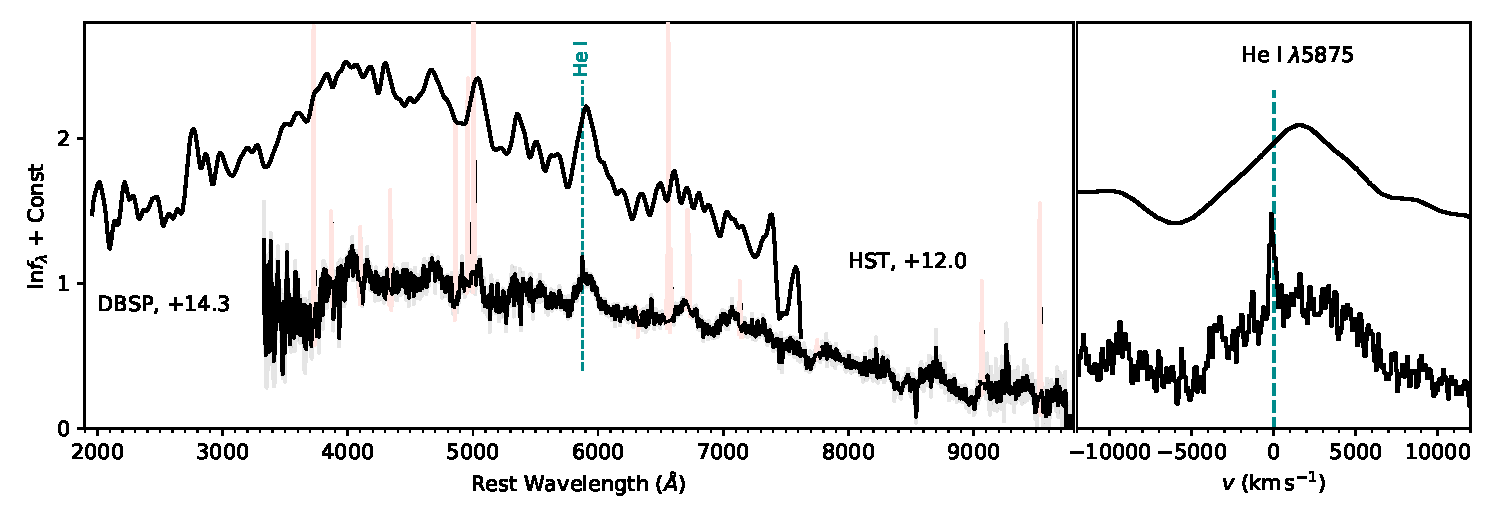
\includegraphics[width=\textwidth]{figures/spectra_phot.pdf}
	\caption{Observed ealy-time and photosperic phase spectra of AT2019dge. For ground-based 
		spectroscopy, the original spectra are	shown in translucent colors, with the overlying black 
		lines showing the same spectra convolved with an 
		${\rm FWHM} = 800\, {\rm km\, s^{-1}}$ (for LT) or ${\rm FWHM} = 200\, {\rm km\, 
			s^{-1}}$ (for DBSP and LRIS) Gaussian kernel. We mask prominent galaxy lines of the 
		DBSP spectrum in light red. In the right panels, we show spectral 
		evolution in velocity space around prominent SN lines, where the $y$-axis is 
		\label{fig:spectra}}
	%
\end{figure*}
\begin{figure*}[htbp!]
	%
	\centering
	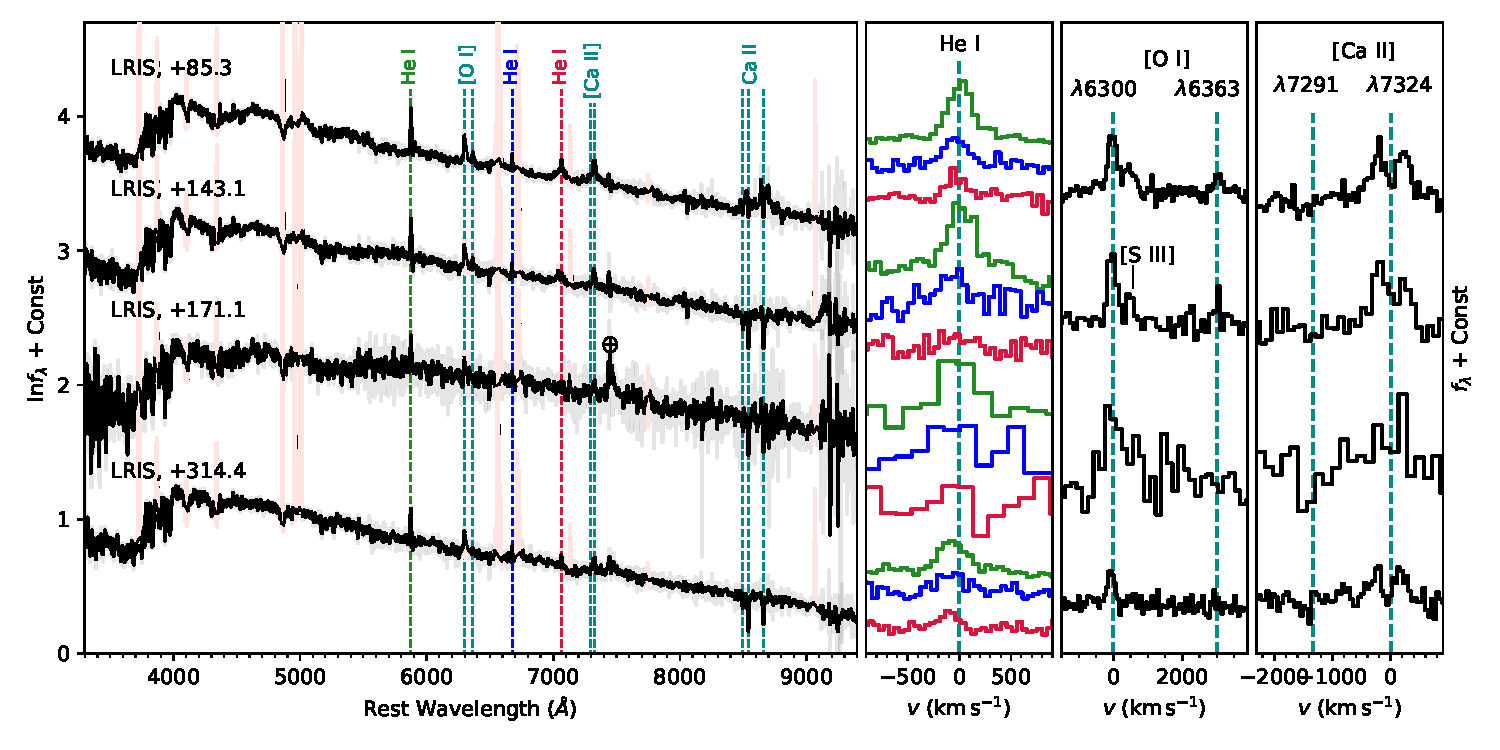
\includegraphics[width=\textwidth]{figures/spectra_late.pdf}\\
	\caption{Observed late-time spectra of AT2019dge. See 
		Figure~\ref{fig:spectra}
		\label{fig:spectra_late}}
\end{figure*}

 
\subsection{Photometry}
\subsubsection{Optical Photometry}
We perform forced PSF photometry on ZTF difference images following the steps illustrated in 
\citet{Yao2019}. The sky region of AT2019dge is covered by two ZTF fields with fieldid 763 and 
1799. We exclude all data in field 1799 since the reference image was constructed using images 
obtained between May 25 2018 and July 12 2019, which is after the explosion of the 
transient\footnote{The ZTF name (ZTF18abfcmjw) indicates that the transient was discovered in 2018. 
However, this is due to a candidate detection from negative subtraction (reference minus science) in 
2018 in field 1799.}.

Since field 763 was included in both the northern sky survey with two epochs (one 
$g\, +$ one $r$) per three nights and the extragalactic high-cadence survey with six epochs (three 
$g\,+$ three $r$) per night\footnote{See \citet{Bellm2019a} for the ZTF experiments design.}, this 
transient are visited muliple times every night. Therefore, single-night flux measurements in the same 
filter are binned (by taking the inverse variance-weighted average). This gives a pre-explosion 
$r$-band limit of 18.95 mag (5$\sigma$ limit computed at the expected position of the transient) on 
April 4 10:36:34. Five-$\sigma$ detections are converted to magnitude for further analysis.

Following the discovery of AT2019dge, we obtained follow-up photometry in $griz$ with the optical 
imager (IO:O) on the Liverpool Telescope (LT; \citealt{Steele2004}). LT and P48 photometry are shown 
in Figure~\ref{fig:lightcurve}. Absolute magnitude is determined by correcting for the distance modulus 
and Galactic extinction $E(B-V)=0.022$ estimated by \citet{Schlafly2011}, which builds upon 
\citet{Schlegel1998}. We assume $R_V=3.1$, and adopt reddening law from \citet{Cardelli1989}. We do 
not correct for host-galaxy contamination given the absence of \ion{Na}{I} D absorption in all spectra 
at the host redshift. 

We also performed forced photometry on archival PTF/iPTF difference images spanning May 07 2009 to 
June 13 2016\footnote{We followed the procedure described in 
	\url{http://web.ipac.caltech.edu/staff/fmasci/home/miscscience/forcedphot.pdf}}. No historical 
detections was found. 
\subsubsection{Swift Photometry}
Space-based observations with the \textit{Neil Gehrels Swift Observatory} (\textit{Swift}; 
\citealt{Gehrels2004}) was triggered on April 9 and April 10. Ultraviolet/Optical Telescope (UVOT; 
\citealt{Roming2005}) data were obtained in the $UVW1$, $UVM2$, $UVW2$, $U$, $B$, and $V$ 
filters. 

UVOT data are reduced using HEAsoft (v6.17) with a $3^{\prime\prime}$ circular aperture. To remove 
host-galaxy contribution at the location of the SN, we obtained a final epoch in all broad-band filters 
on June 23 2019 and measured the photometry with the same aperture used for the transient. We 
present a table of our optical and UV photometry in Section \ref{subsec:appphot_data}.

We note that no point sources were detected in the XRT event files with $\rm{SNR}>2$.
The 3$\sigma$ limits in count\,s$^{-1}$ in the April 9, April 10, and June 23 observations are $7.8\times 
10^{-3}$,  $5.8\times 10^{-3}$, and $6.1\times 10^{-3}$, respectively.

\subsubsection{Radio Follow-up}
We observed at high frequency radio bands using the Submillimeter Array (SMA, \citealt{Ho2004}) on 
UT 2019 xx xx under its target-of-opportunity program. The project ID was xxx. Obser \todo{finish this}


\subsection{Spectroscopy}

We obtained eight optical spectroscopic follow-up of AT2019dge from $-1.1$\,d to $+314.4$\,d relative 
to $g$-band peak using the Rapid Acquisition of Transients (SPRAT; \citealt{Piascik2014}) on the 
Liverpool Telescope (LT), the Double Spectrograph (DBSP) on the 200-inch Hale telescope 
\citep{Oke1982}, and the Low Resolution Imaging Spectrograph (LRIS) on the Keck-I telescope 
\citep{Oke1995}. We use the automated LT pipeline reduction and extraction for the LT spectra. The 
DBSP spectrum was reduced using a \texttt{PyRAF}-based reduction pipeline \citep{Bellm2016}. LRIS 
spectra were reduced and extracted using \texttt{Lpipe} \citep{Perley2019lpipe}. 


An HST slitless NUV spectrum was obtained at phase $+12.0$\,d as part of our HST program 
(GO-15675, PI Fruchter) using the WFC3 G280 grism. We obtained a short (60\,s) direct image of this 
field in the F300X filter to  set  the wavelength scale of the  spectrum. We also obtained  a longer 
exposure (200\,s) in the F350LP filter (see Figure~\ref{fig:offset}), which has very similar throughput to 
the zeroth order of the G280 grism. We convolved this image to match the slight blurring of the 
zeroth order G280 grism and then scaled and subtracted it, dramatically reducing host contamination 
from the zeroth order host image.
%70@300nm and an average dispersion of about 1.3 nm per pixel 

A log of our spectroscopic observations is presented in Appendix \ref{subsec:appspec_data}. We 
present our sequence of spectra in Figure~\ref{fig:spectra} and Figure~\ref{fig:spectra_late}.

\section{Properties of the Explosion \\and Its Host Galaxy}
\subsection{Light Curve Properties}\label{subsec:lc_properties}

\subsubsection{Peak Luminosity, Rise and Decline Timescale}
To estimate the epoch of maximum light, we interpolated the $g$- and $r$-band photometry with 
three-order polynomial functions, as is shown in the inset of Figure~\ref{fig:lightcurve}. The time range 
used in the fit is from ${\rm MJD}=58581.2$ to $58585.2$. AT2019dge was found to peak 
at $M_{g\rm , peak}=-16.45\pm0.04$ mag on ${\rm MJD}=58583.19$, and $M_{r \rm ,peak } 
=-16.27\pm0.02$ mag on ${\rm MJD}=58583.39$. Hereafter we use phase ($\Delta t$) to denote time
with respect to the $g$-band maximum light epoch, ${\rm MJD}=58583.2$.

The $g$- and $r$-band peak luminosity of AT2019dge ($\approx -16.3$\,mag) is around the lower limit 
of stripped envelope SNe, and more similar to those of the Ca-rich gap transients, 
which occupy the luminosity `gap' between novae and SNe (peak absolute magnitude $M_R \approx 
-15.5$ to $-16.5$\,mag).

\begin{figure}[htbp!]
	\centering
	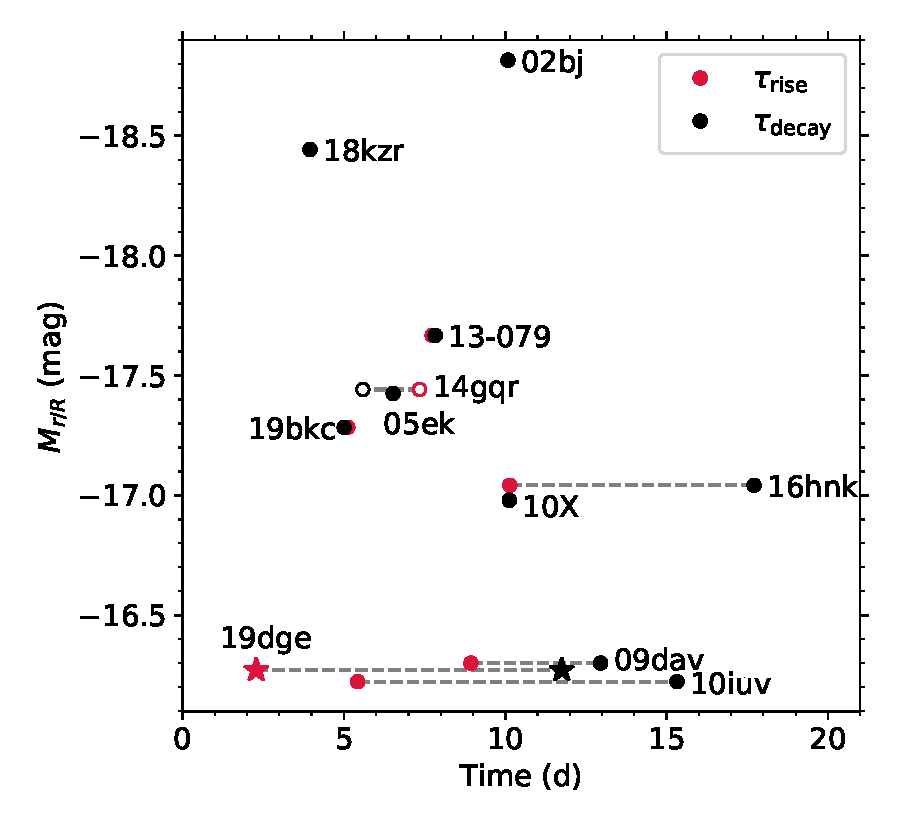
\includegraphics[width=\columnwidth]{figures/compare_mag.pdf}
	\caption{Comparison of the photometric evolution timescales ($t_{\rm rise}$ and $t_{\rm  
			decay}$) and peak absolute magnitude of AT2019dge to other H-deficient fast-evolving 
		These include 
		SN2002bj \citep{Poznanski2010},
		SN2005ek \citep{Drout2013},  
		PTF09dav \citep{Sullivan2011},
		SN2010X \citep{Kasliwal2010},
		PTF10iuv \citep{Kasliwal2012},
		iPTF14gqr \citep{De2018},
		KSN2015K \citep{Rest2018},
		 iPTF16asu	\citep{Whitesides2017}, 
		 iPTF16hgs \citep{DeKC2018},
		SN2018gep \citep{Ho2019},
		SN2018kzr \citep{McBrien2019}, 
		and SN2019bkc \citep{Chen2020}. 
		For the two SNe with double peaked light 
		curve (iPTF14gqr and iPTF16hgs), $t_{\rm rise}$ is estimated from model fitting to the first peak 
		since the rise of first-peak was not observed, and $t_{\rm decay}$ is estimated from the decline of 
		the second peak. Peak magnitude is given in $r$-band, except for KSN2015K where we 
		only have observations in the \textit{Kepler} white filter, and iPTF16asu where the rise was only 
		caught in $g$-band (but in rest-frame $r$-band since this is a high-redshift event).
		%\\ZTF $g$-band detection for SN2019bkc and ATLAS $o$-band detection for SN2016hnk. 
		\label{fig:compare_mag}}
\end{figure}


To characterize the rise and decline timescales of AT2019dge, we calculate rise time ($t_{\rm rise}$) 
defined by how long it takes the $r$-band light curve to rise from one magnitude below peak to peak, 
and decline time ($t_{\rm decay}$) determined by how long it takes to decline from peak by one 
magnitude. In Figure \ref{fig:compare_mag} we compare the rise time, decay time, 
and peak absolute magnitude between AT2019dge and other fast-evolving hydrogen-deficient 
transients from the literature. 

It is clear from the upper panel that AT2019dge rose faster than normal Ca-rich events such as 
PTF09dav and PTF10iuv. The rise time of $\approx 2$\,d is similar to some fast evolving luminous 
transients (FELTs) such as KSN2015K, iPTF16asu, and SN2018gep, but its substantially low luminosity 
suggests that AT2019dge is physically distinct from the class of FELTs. In the subluminous regime, 
iPTF14gqr and iPTF16hgs have $t_{\rm rise}$ comparable to AT2019dge. Both transients exhibit 
double-peaked light curve where the first peak is postulated to be caused by the diffusion of 
shock-deposited energy out of an envelope around the progenitor star.
 
The bottom panel of Figure \ref{fig:compare_mag} shows that $t_{\rm decay}$ of AT2019dge is 
longer than many well-observed rapid-fading Type Ib/c SNe, such as SN2002bj, SN2018kzr, SN2005ek, 
and SN2019bkc. Its decay timescale is more similar to SN2010X, iPTF14gqr, as well as the population of 
Ca-rich transients PTF09dav, PTF10iuv, and iPTF16hgs. It has been suggested that the latter group of 
events have radioactivivity powered main peak with low mass of nickel ($M_{\rm Ni} \lesssim 0.1 
M_\odot$).

We conclude that the AT2019dge is not one of FELTs. Its fast $t_{\rm rise}$ is reminiscent of shock 
cooling emission, and the moderate $t_{\rm decay}$ is consistent with coming from radioactivity.

\subsubsection{Bolometric Evolution}
\begin{figure}[!htbp] 
	\centering
	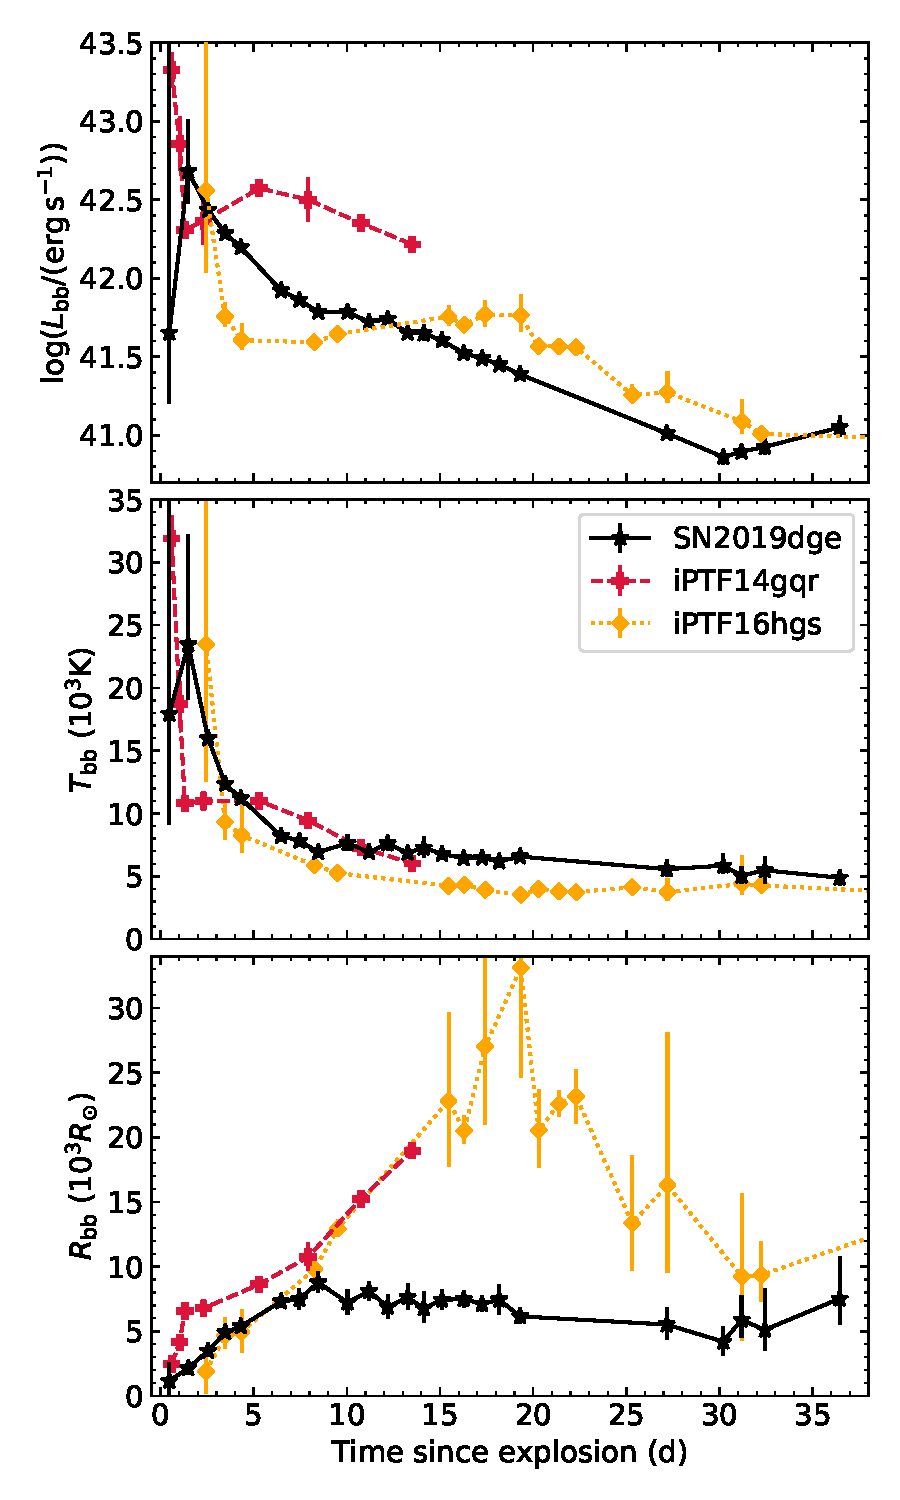
\includegraphics[width=\columnwidth]{figures/Tbb_Rbb.pdf}
	\caption{Evolution of blackbody properties (lumionosity, temperature, radius) over time of 
		AT2019dge compared to iPTF14gqr and ZTF18aalrxas.}
	\label{fig:Tbb_Rbb_Lbb}
\end{figure}

We constructed the bolometric light curve evolution by fitting a blackbody function to the spectral 
energy distribution (SED). At eighteen epochs where at least detections in three flters are available, we 
utilized the Monte Carlo Markov Chain (MCMC) simulations with \texttt{emcee} 
\citep{Foreman-Mackey2013} and adopted wide and flat prior for the blackbody radius and 
temperature ($0<T_{\rm bb}<10^6$\,K, $0<R_{\rm bb}<10^6\,R_\odot$). Uncertainties are estimated 
using the difference between the 84th and the 16th percentiles of posterior probability distributions. At 
five epochs that we only have photometric observations in two filters, we fit for $T_{\rm bb}$ and 
$R_{\rm bb}$ with no estimates on the parameter uncetainties. The SED fits are shown in 
Appendix \ref{subsec:appphot_data}. 

Adopting the explosion epoch estimated in Section \ref{subsec:fastrise} at $\Delta t=-3.20$\,d (i.e., 
0.46\,d before the discovery epoch), we plot the physical evolution in Figure~\ref{fig:Tbb_Rbb_Lbb}, 
with a comparison to peculiar SN Ic iPTF14gqr \citep{De2018} and stripped envelope SN IIb 
ZTF18aalrxas \citep{Fremling2019}. The bolometric luminosity peaks at $ t=1$--2\,d 
after the assumed explosion epoch, at $\sim 5\times 10^{42}\,{\rm erg\, s^{-1}}$. The initial fast drop of 
luminsity ($0.36\,{\rm mag\,d^{-1}}$) and temperature is similar to the early evolution of several 
stripped envelope SNe displaying double-peaked light curve, where the first peak has been modelled 
by cooling emission from an extended envelope around the progenitor after the core-collapse SN 
shock breaks out \citep{Modjaz2019}. We interpret the early evolution in the context of shock-cooling 
emission in Section \ref{subsec:fastrise}.

The lumnosity falls at a much slower rate at later times ($ t \gtrsim 9$\,d) while the radius remains flat. 
The total integrated blackbody energy output during $ t = 0.6$--30\,d is $\sim 
2\times 10^{43}\,{\rm erg\,s^{-1}}$. Assuming that the photospheric radius linearly expands at early 
phase, we fit a linear function to the $R_{\rm bb}$ vs.~$\Delta t$ diagram (bottom panel of 
Figure~\ref{fig:Tbb_Rbb_Lbb}). 

\subsubsection{Color Evolution}
\begin{figure*}[htbp!]
	\centering
	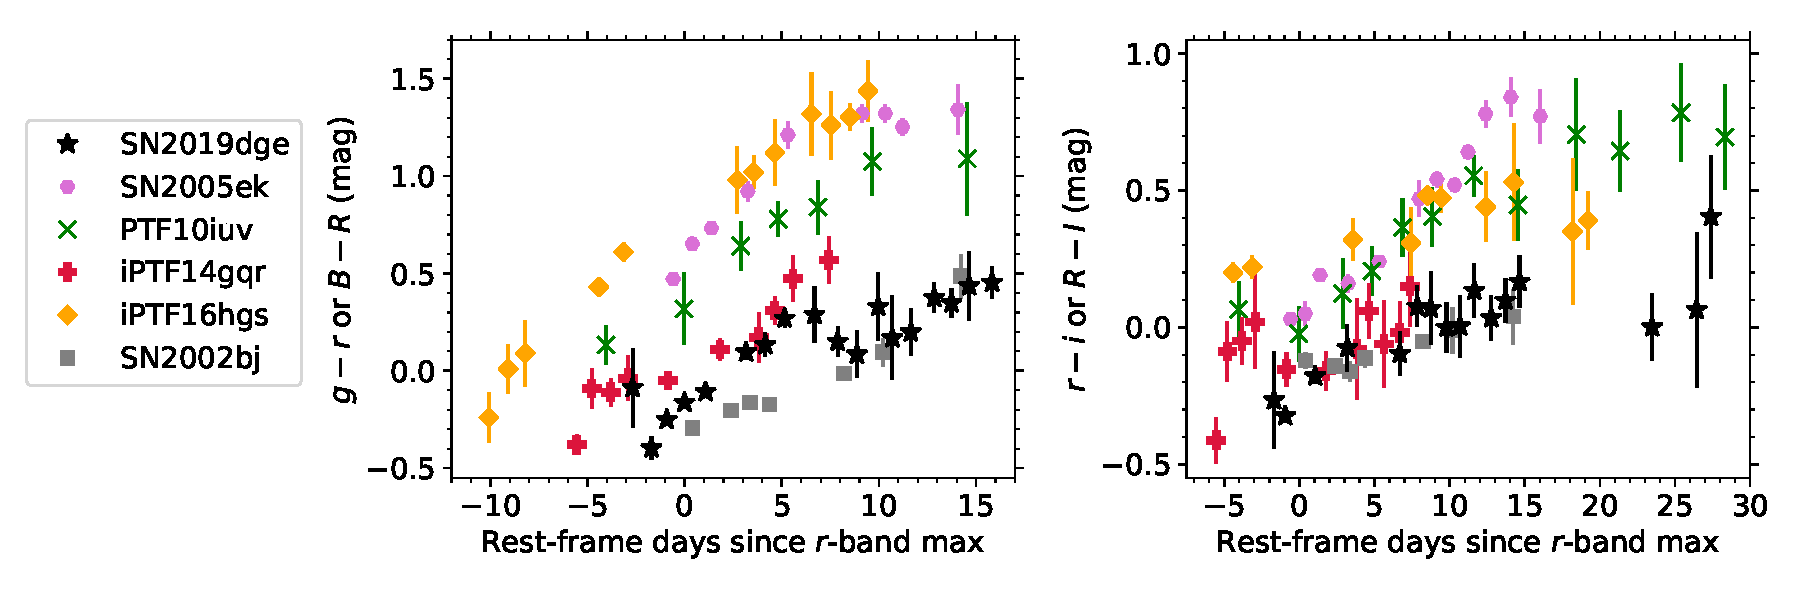
\includegraphics[width=\textwidth]{figures/compare_color.pdf}
	\caption{Comparison of the color evolution of AT2019dge with some other fast SNe shown in 
		Figure~\ref{fig:compare_mag}. All colors have been corrected for Galactic extincton. Due to 
		absence of photometry in identical filters, we compare colors in corresponding filter pairs of 
		$B$/$g$, $R$/$r$ and $I$/$i$.  \label{fig:compare_color}}
\end{figure*}
We compare the color curves of other fast transients to that of AT2019dge in 
Figure~\ref{fig:compare_color}, in corresponding pairs of $B$/$g-R$/$r$ and $R$/$r-I$/$i$ colors. For 
double-peaked events iPTF14gqr and iPTF16hgs, ``maximum'' time corresponds to epoch of maximum 
light in the second peak.

The 
early-time blue color of AT2019dge arises from the high-temperature peak. Subsequently, AT2019dge 
has relatively typical $g-r$ color evolution among this set of transients, displaying a 
progression from a very blue transient ($g-r \approx -0.4$ mag) at early times to a relatively red 
transient ($g-r \approx 0.5$) within 10 days of explosion. This fast reddening is indicative of rapid 
cooling of the ejecta since the spectra at these phases are broadly consistent with featureless 
continua. We conclude that the multi-color light curves of the main peak of iPTF 14gqr exhibit several 
similarities (light curve shape and timescales) as well as unique differences (short rise time) in this 
sample of transients.

AT2019dge shows a color starting out blue and turning redder with time, consistent with an expanding 
and cooling photosphere.

Although AT2019dge has the same optical peak luminsity as Ca-rich transients, their multi-color light 
curves of are very different in shape. The color evolution  which otherwise form a fairly homogeneous 
class. 

\todo{AT2019dge is special in that the color even turned green a littble bit at $6<\Delta t<10$.}


\subsection{Spectroscopic Properties}\label{subsec:spec_properties}
\subsubsection{Early Spectral Evolution}

The very early spectra at $-1.1$, $-0.1$, and $+0.4$\,d show a blue continuum and strong galaxy 
emision lines from the underlying \ion{H}{II} region (see the top panel of Figure~\ref{fig:spectra}). In 
addition, these spectra also show prominent \ion{He}{I} $\lambda5875$ and high-ionization \ion{He}{II} 
$\lambda4686$ narrow emission lines ($\sim 600\,{\rm km\,s^{-1}}$). The low-velocity flash lines are 
not coming from the fast SN ejecta but rather from photoionized material in a region of undistrubed 
CSM exterior to the SN \citep{Leonard2000}. Using the line index definition given by 
\citet{Khazov2016}, we calculated the equivalent width of \ion{He}{II} to be $-7.56\pm 1.07$ $-2.66\pm 
1.30$, and $-3.77\pm 0.16$ in the $-1.1$\,d, $-0.1$\,d, and $+0.4$\,d spectra.

\todo{rewrite this: If the exploding star is embedded in circumstellar material (CSM) that is dense (n∼ 
1012 cm−3) and extended (r> 1013 cm), the CSM will be flash-ionized and quickly recombine, imprinting 
a strong emission-line pattern onto the underlying hot continuum. Eventually, the expanding SN ejecta 
plow through any nearby CSM (moving at typical expansion velocities of 104 km s−1, SN ejecta cover ∼ 
9×1013 cm per day) and wipe out the emission-line spectrum, transforming it into a blue, featureless 
continuum that is typical for few-day old SN spectra;}
These lines were created by recombination of some CSM flash-ionized by a shock breakout 
\citep{Khazov2016}

We make an order-of-magnitude estimate on the progenitor mass-loss rate following the xx given by 
\citet{Ofek2013}


\begin{figure*}[htbp!]
	\centering
	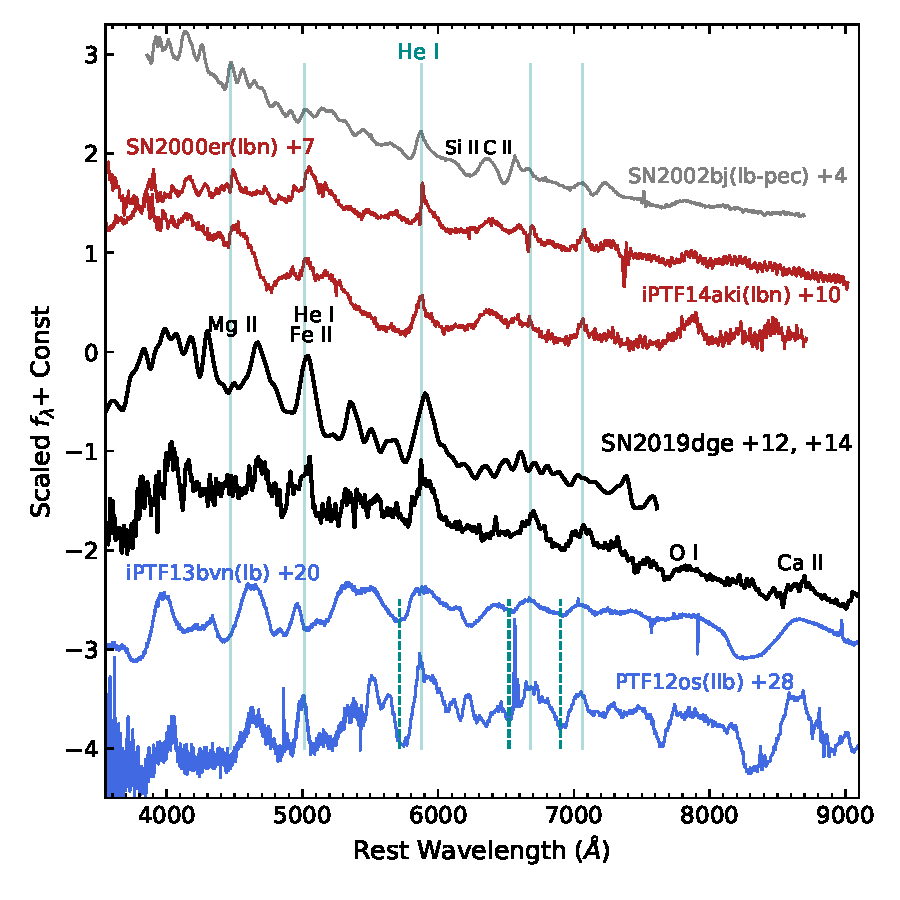
\includegraphics[width=0.495\textwidth]{figures/hst_opt.pdf}
	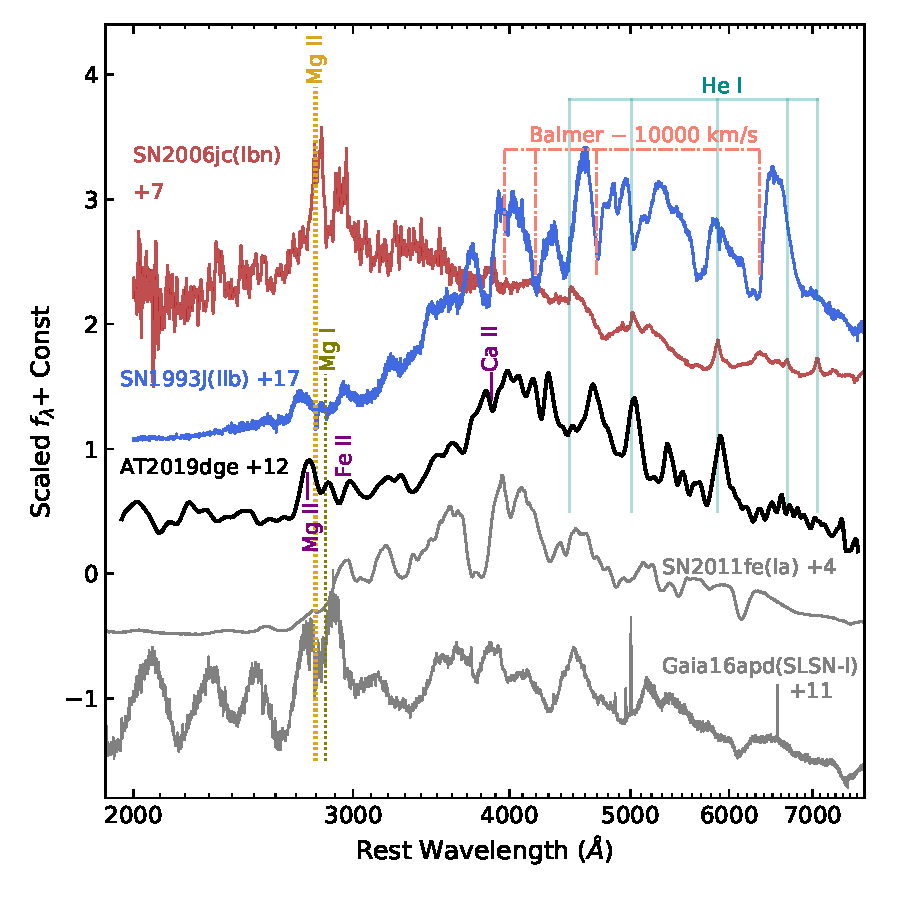
\includegraphics[width=0.495\textwidth]{figures/hst_all.pdf}
	\caption{$Left$: AT2019dge compared with spectra of 
	other SNe, 
	including SN2002bj \citep{Poznanski2010}, SN2005bf \citep{Folatelli2006}, SN2008ax 
	\citep{Chornock2011}, PTF12os and iPTF13bvn \citep{Fremling2016} \todo{include iPTF10iuv??? 
	iPTF16hgs??? }
	$Right$: HST spectrum of AT2019dge compared with spectra of other SNe, including SN2006jc 
	\citep{Bufano2009}, SN1993J \citep{Jeffery1994}, SN2011fe \citep{Mazzali2014}, and Gaia16apd 
	\citep{Yan2017}.
		\label{fig:hst}}
\end{figure*}
\subsubsection{Photosperic Phase Spectral Evolution}
Broad transient features show up in the $+12.0$ adn $+14.3$\,d spectra. The existence of P-Cygni 
\ion{He}{I} $\lambda5876$ profile and non-existence of hydrogen is reminiscent of Type Ib 
SN. The HST spectrum should contain little host-galaxy contamination due to its narrow 
slitwidth and high resolution, otherwise we should see emission features at prominent galaxy line 
wavelengths (H$\alpha$, [\ion{O}{III}], [\ion{O}{II}], etc). The UV part is much weaker than a blackbody 
extrapolation opf their optical spectra would predict. This has also been seen in previous UV 
observations of SNe, and interpreted as strong metal-line blanketing, mostly by \ion{Fe}{II} and 
\ion{Co}{II} lines \citep{Gal-Yam2008}.

\todo{say that the undulations at 6700\AA is likely just noise. Ask David to put a trace on the galaxy 
center and show spectrum to get a sense of the SNR}

In Figure~\ref{fig:hst_opt} we show that AT2019dge share similarity with those of normal SNe Ib/IIb in 
the optical region, but the spectrum does not match any known SN in 4000-4500\AA\,and 
6500--7500\AA. In Figure~\ref{fig:hst_all} we compare the HST UV spectrum too other type of SN. 
AT2019dge most closely resemble SN1993J between 2000 and 4000\AA. .

Enhanced (and potentially eruptive) mass-loss during the final stages of stellar evolution is a key probe 
of poorly understood physics (e.g., Shiode \& Quataert 2013; Smith \& Arnett 2014) that sets the initial 
conditions to core-collapse. 

We measure the velocity of the \ion{He}{I} $\lambda5876$ line by fitting a parabola to the absorption 
minimum. This resulting fits give a velocity of $\approx 6000\, {\rm km\,s^{-1}}$ and $ 5900\, {\rm 
km\,s^{-1}}$ for the $+12.0$\,d and $+14.3$\,d spectra, respectively; At maximum light, we expect the 
photospheric velocity to be higher. A linear fit to the first few $R_{\rm bb}$ vs. time measurements 
(lower panel of Figure \ref{fig:Tbb_Rbb_Lbb}) gives $\approx 8150\, {\rm km\,s^{-1}}$. Hereafter we 
assume the ejecta velocity to be $v_{\rm ej} = 8150\, {\rm km\,s^{-1}}$


\todo{consider use Marc Williamson 2019 paper to confirm the peculiarity of this event}

The UV emission fades with time from explosion as the photosphere cools and line blanketing from 
metals becomes important in this part of the spectrum (particularly Fe II and Fe III; see M00; DH05, 
DH06). Thus when reached by HST about two weeks after burst, the UV and blue optical spectrum of 
the supernova is dramatically altered by the metal content of the ejecta at the line forming region.   In 
particular, the combination of both UV and optical spectra allows us to break degeneracy between 
temperature and metallicity. 

Ba03:  Baron, E., et al.2003, ApJ, 586, 1199
%M00:  Mazzali, P. A.2000, A&A, 363, 705
%D05:  Dessart, L., & Hillier, D. J. 2005, A&A, 437, 667
%DH06:  Dessart, L., & Hillier, D. J. 2006, A&A, 447, 691

 On the other hand, the limited number of UV spectra of Type Ib/c SNe have revealedconsiderable 
 differences – while the Type Ib SN 1983N (P03) showed several similarities toType Ia SNe in its UV 
 spectrum, the Type Ib SN 2006jc appeared to exhibit emission linesof likely Mg II features, suggested 
 to be associated with interaction of the SN ejecta witha pre-exisiting CSM wind.  In these cases, 
 ionization of the wind material by the SN shockwave can produce emission features of highly ionized 
 elements (e.g.  N V, N III and Si IV) aspreviously suggested in UV spectrum modeling of older events 
 (SN 1979C and SN 1980K;Be82; Pa80; Fr84).  Thus, UV spectra of core-collapse SNe are also a 
 powerful probe of in-teraction between the SN ejecta and a pre-existing CSM around the progenitor, 
 constrainingthe pre-explosion mass loss history of the progenitor stars

\subsubsection{Late-time  Spectral Evolution}
\begin{figure*}
		\centering
	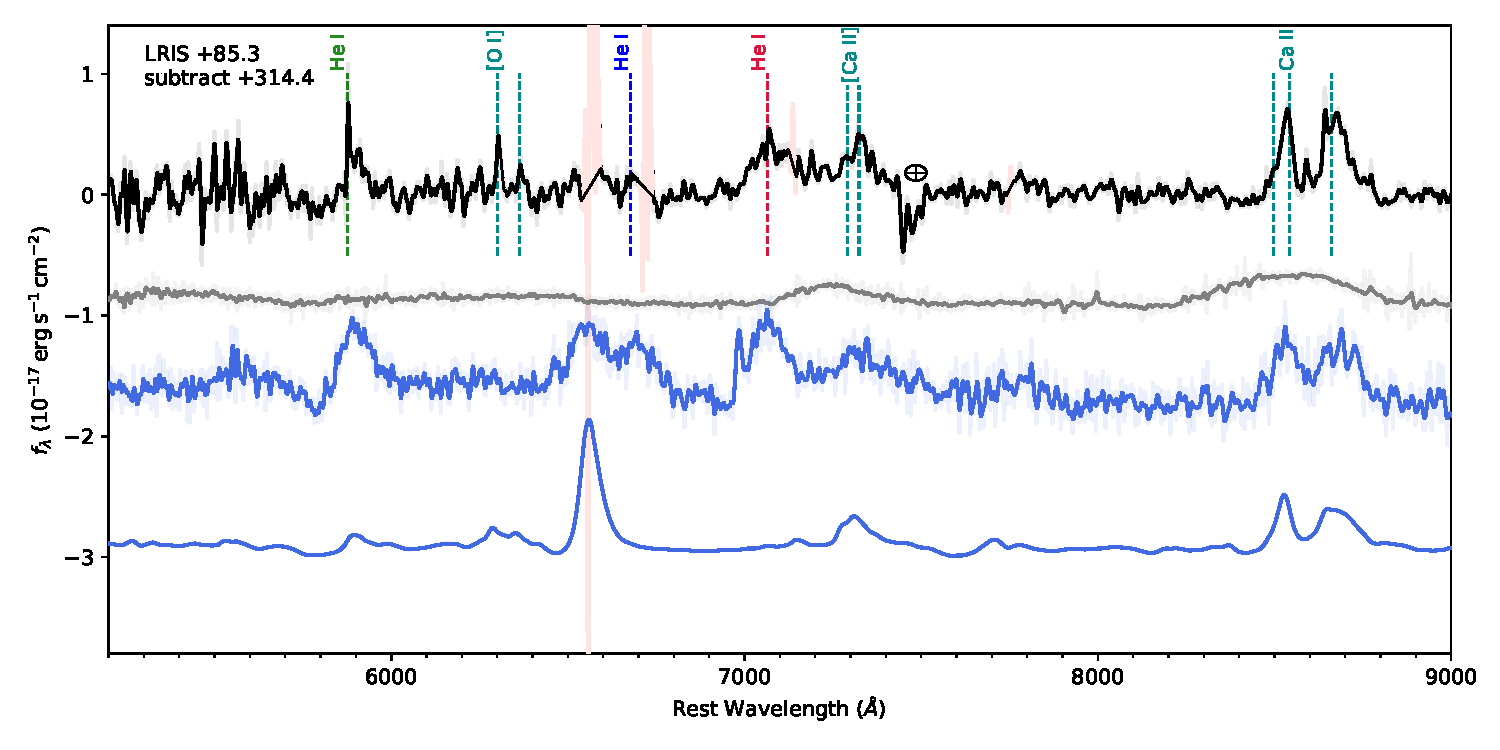
\includegraphics[width=\textwidth]{figures/spec_host_subtracted.pdf}
		\caption{some caption}
\end{figure*}
In our late time spectrum obtained at $+85.3$, $+143.1$ and $+171.1$\,d, we observe narrow emission 
lines that are typically the most prominent features of SNe Ib/c at nebular epochs. The emission feature 
at $\sim6300$\AA\,is regularly attributed to [\ion{O}{I}] $\lambda\lambda$6300, 6364 
\citep{Maedo2008}

\ion{O}{I}, \ion{Ca}{II} and \ion{He}{I} lines. 
This feature is , and  (e.g., Maeda et al. 2008; Taubenberger et al. 
2009). The presence or absence of this feature has often been considered the sharpest observational 
discrimination between core-collapse and thermonuclear SNe (e.g., Filippenko 1997). 
the [O i] λλ6300, 6364 feature consists of two similarly strong, fairly narrow emission peaks on top of 
a broad base (figure blah blah)

In Figure \ref{fig:HeI_dbsp} we show the 
Its absorption minimum indicates a velocity of xxx

only three months after maximum light, a spectrum taken with LRIS
The timescale to become nebular was surprising as it was faster than that of typical supernovae by a 
factor of a few.

\subsection{Host Galaxy Properties}
In Figure~\ref{fig:offset}, we show the source position on the image from the Beijing-Arizona Sky 
Survey(BASS, \citealt{Zou2017}), which is part of the DESI Legacy Imaging Surveys \citep{Dey2019}. 
Using the xx, we calculated 
that AT2019dge is $0.14^{\prime\prime}$ (0.06\,kpc) away from the galaxy nucleus, which is defined to 
be the flux-weighted first 
moment of the BASS $g$-band image.

Since there was no pre-explosion spectrum of the host galaxy, we estimated the host flux 
by fitting a synthetic galaxy spectrum with SDSS model magnitudes (van Velzen et al. 2019). To 
perform subtraction of the host flux, we calibrated the flux level in each optical spectrum against ZTF 
$r$-band photometry, interpolated to the spectroscopic epochs. We then convolved the synthetic 
host galaxy spectrum new
Gaussian kernel to account for instrumental broadening and subtracted 
the broadened, synthetic spectrum from our observed spectra. A montage of the host-subtracted 
spectra is shown in Figure \ref{fig:spectra}. The flux is normalized to the 5500–6000 A ̊ region in rest 
wavelength and offset from each other for better visualization.

In Fig we shoulw the SED of xx, which was compiled from Swfit/UVOT, SDSS, and catalogs and 

We measure the metallicity of the host galaxy using  the spectrum xx. 

We infer a star-formation rate of $0.10 \pm 0.02 \, M_\odot\, {\rm yr^{-1}}$ from the H$\alpha$ 
emission line using the \citet{Kennicutt1998} relation converted to use a Chabrier initial mass function 
\citep{Chabrier2003, Madau2014}. 

We also compute the oxygen abundance using the strong-line metallicity indicator N2 
\citep{Pettini2004} with the updated calibration reported in \citet{Marino2013}. The oxygen abundance 
in the N2 scale is 8.23 $\pm$ 0.01 (stat) $\pm$ 0.05 (sys).

\textcolor{red}{Zhihui:} 
We further determine the stellar mass ($M_{\star}$) of the host galaxy by SED modeling using 
\texttt{CIGALE} \citep{CIGALE19}. We adopt the stellar population synthesis models from \citet{BC03} 
with the Chabrier IMF \citep{Chabrier2003}, and assume a double declining  exponential star formation 
history (SFH). In addition, a dust component is added using the \citet{DL07} model to account for dust 
emission. Finally, the total SED model is attenuated by the Calzetti extinction curve \citep{Calzetti2000}.

The fitted SED is shown in Figure 7. The derived stellar mass is log $M_{\star}/M_{\odot}$ = 
$8.0 \pm 0.1$, and the SFR is $0.8 \pm0.1\, M_\odot\, {\rm yr^{-1}}$.

\begin{figure*}[htbp!]
	\centering
	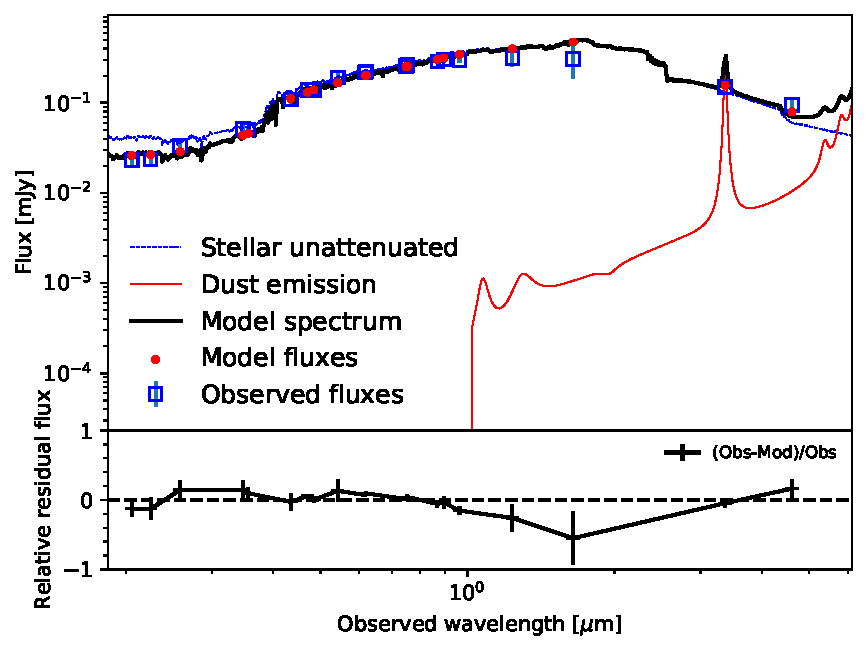
\includegraphics[width=1.2\columnwidth]{figures/SDSSJ17+50_best_model.pdf}
	\caption{Spectral energy distribution of the host galaxy of AT2019dge. The observed photometric 
	data (with 1$\sigma$ error bars) are shown in blue open squares, and the model is shown in black 
	curve. The relative residual flux is shown in the bottom panel.
		\label{fig:SEDfit}}
\end{figure*}

It is worth noting that while several 
previously reported events (SN\,2005ek, SN\,2010X, iPTF\,14gqr) and SN\,2018kzr were found in star 
forming host galaxies, SN\,2019bkc stands out as a hostless transient offset by tens of kpc from any 
likely host (see Table \ref{tab:compare}). 


\subsection{Spectroscopy}

Although there is a large diversity in the properties of these events, most of them can be 
grouped into events that are similar to thermonuclear SNe (e.g. PTF09dav, \citealt{Sullivan2011}; 
OGLE-2013-SN-079, \citealt{Inserra2015}; SN2016hnk, \citealt{Galbany2019, Jacobson-Galan2019}) 
likely arising from old white dwarfs, and those similar to Type Ib/c SNe (SN\,2002bj, 
\citealt{Poznanski2010}; SN\,2005ek, \citealt{Drout2013}; SN\,2010X, \citealt{Kasliwal2010}; iPTF\,14gqr, 
\citealt{De2018}) possibly arising from extremely stripped massive stars or white dwarfs in close binary 
systems.

Ca-rich transients have detectable [O I] λλ6300, 6364 emission in nebular spectra, but a defining 
feature of the class is an integrated [Ca II]/[O I] flux ratio greater than ∼2. 

\subsection{Host Environment}

Table \ref{tab:compare} shows a summary of our literature search.

\begin{deluxetable*}{lllll}[htbp!]
	\tablecaption{Summary of Subluminous Fast Transient. \label{tab:compare}}
	\tablehead{
		\colhead{Name}   
		& \colhead{Redshift} 
		& \colhead{Host} 
		& \colhead{Offset (kpc)}   
		& \colhead{Reference}   
	}
	\startdata
	SN\,2002bj & 0.012   & NGC 1821 (small barred irregular galaxy, $D\sim$1.1'') & 1.8\,kpc \\
	SN\,2005ek & 0.016 & UGC 2526 (edge-on spiral galaxy of morphology Sb) & 30\,kpc \\
	% SN 2007ax, from the SDSS image, I think it is 5 arcsec from the host
	SN\,2007ax & 0.007  & NGC 2577 (small lenticular galaxy with a condensed core) &1.0\,kpc 
	\\
	PTF\,09dav & 0.036& spiral galaxy & $\sim40.6$\,kpc\\
	SN\,2010X &  0.015  & NGC 1573A (small spiral galaxy, $D\sim$1.6'') & 2.3\,kpc\\
	%PTF\,10iuv & 0.025?   &  Galaxy cluster with early-type and late-type galaxies   & $\geq 37$\,kpc  \\
	OGLE13-079 & $\sim$0.07  & in the extreme outskirts of two ellipticals & 40.2--49.9\,kpc \\
	iPTF\,14gqr & 0.063 & IV Zw 155 (a tidally interacting spiral galaxy) & 29\,kpc & \citet{De2018} \\
	SN\,2016hnk & 0.016 & MCG-01-06-070 (Sb-type galaxy)  & 3.71 & \citet{Galbany2019}\\
	% SN2018kzr (ZTF18adaykvg), host is SDSS J082853.50$+$010638.6, offset D = d_A \times \theta = 
	%d_L / (1+z)^2 \times \theta
	SN\,2018kzr & 0.053  &  SDSS J082853.50$+$010638.6 (star forming galaxy)   &  0.6 & 
	\citet{McBrien2019}\\
	SN\,2019bkc & $\sim$0.02   & maybe NGC 3090 (giant elliptical in the MKW1 galaxy group) 
	&$\sim94.6$ & \citet{Chen2019}  \\
	AT2019dge & 0.021 & SDSS J17$+$50 (small) & 0.06 kpc & This work \\
	%ZTF\,18abkmbpy & 0.029 (129\,Mpc) &  &   kpc \\
	\enddata
	%\tablecomments{Reference: SN\,2019bkc \citep{Prentice2019}, iPTF\,14qgr \citep{De2018}, 
	%OGLE13-079 \citep{Inserra2015}, SN\,2002bj 
	%\citep{Poznanski2010}, SN\,2010X \citep{Kasliwal2010}, SN\,2016hnk \citep{Galbany2019}, 
	%AT\,2018dge (Yao in prep), SN\,2005ek \citep{Drout2013}.}
\end{deluxetable*}

\clearpage

\section{Interpretation}
\subsection{Shock Cooling Powered Fast Rise} \label{subsec:fastrise}
SNe light cuves are mainly powered by shock energy or radiative diffusion from a heating 
source. We first examine if the peak of AT2019dge is likely to be powered by the radioactive decay of 
$^{56}\rm Ni \rightarrow ^{56}Co \rightarrow ^{56}Fe$. With power a peak luminosity of $L_{\rm 
peak}\approx 5\times 10^{42}\,{\rm erg \, s^{-1}}$ and a rise time of  $t_{\rm peak}\approx 2$--$4\,{\rm 
d}$, AT2019dge falls into the unshaded region of \citet[][Fig.~1]{Kasen2017}, where an unphysical 
condition of $M_{\rm Ni} > M_{\rm ej}$ is required. Therefore, we rule out radioactive decay as the 
power source for the fast rise of the light curve.

Next, we model the early light curve as cooling emission from shock-heated extended material, which 
locates at the outer layers of the progenitor or outside of the progenitor. We use models presented by 
\citet[][hereafter P15]{Piro2015} to constrain the mass and radius of the extanded material ($M_{\rm 
ext}$ and $R_{\rm ext}$, respectively), where $M_{\rm ext}$ includes only mass concentrated around 
$R_{\rm ext}$. This model is built on analytical results of \citet{Nakar2014}. Details of the model fitting 
to multi-band observations are illustrated in Appendix \ref{subsec:p15fit}. 
\begin{figure}
	\centering
	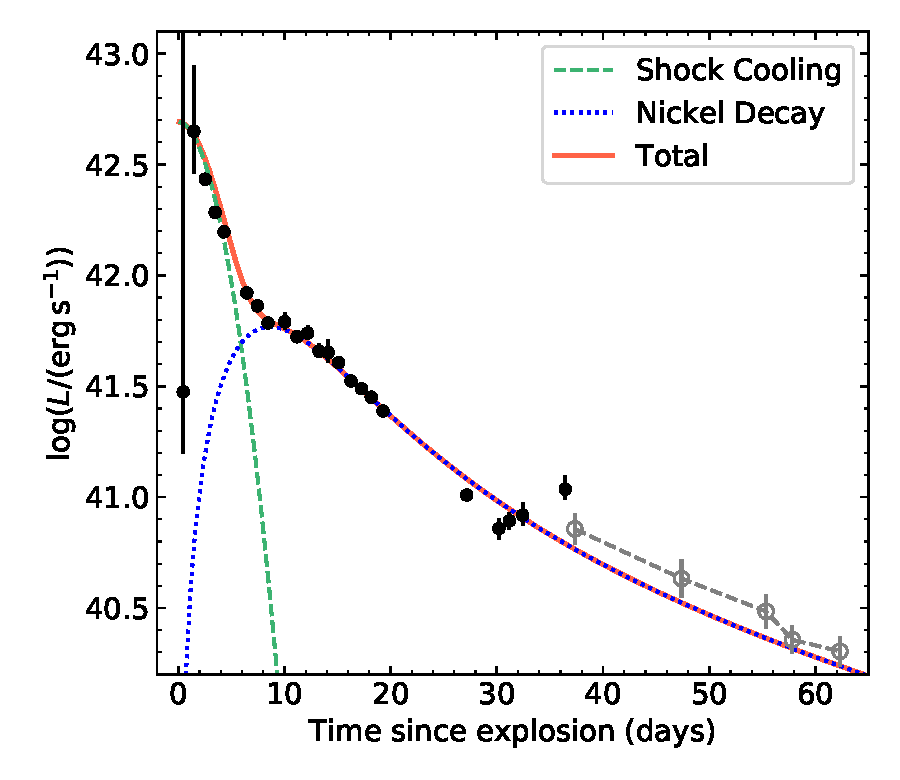
\includegraphics[width=\columnwidth]{figures/Lbb.pdf}
	\caption{Bolometric light curve for AT2019dge. The quasi-bolometric light curve of AT2019dge 
	estimated by computing $\nu L_\nu$ in $r$-band is shown as emply grey circles. The dashed green 
	and dotted blue lines show the best fits of shock cooling and nickel decay models. The solid red line 
	shows the combination of the two components.}
	\label{fig:Lbb}
\end{figure}

In Figure~\ref{fig:Lbb}, bolometric light curve measured in Section \ref{subsec:lc_properties} are shown 
in black. We also show late-time $r$-band $\nu L_{\nu}$ measurements in grey empty circles as a 
proxy of bolometric light curve evolution. The dashed green line  shows the best-fit model of 
$M_{\rm ext} = 9.40_{-0.33}^{+0.35}\times 10^{-2} M_\odot$, $R_{\rm ext} 
=2.69_{-0.16}^{+0.18}\times10^{12}$\,cm (i.e., $38.7_{-2.4}^{+2.5} R_\odot$), and first light epoch at 
phase $t_{\rm fl}= -3.20_{-0.04}^{+0.03}$\,day (i.e., the explosion occurred 0.44\,d before the first 
detection in $g$-band).

Given the simple assumptions of the model, we expect the constraints on $M_{\rm ext}$ and $R_{\rm 
ext}$ to be only approximatedly accurate. There are now numerous cases of early cooling envelope 
emission observed in CCSNe, where the extented matrial is estimated to have lower mass ($\sim 
0.001$--$0.01 M_\odot$) and larger radius ($\sim 10^{13}\, {\rm cm}$) compared to AT2019dge 
\citep{Modjaz2019}. We thus conclude that the early shock cooling emission was produced by an 
extended shell (instead of an envelope) with a mass of $\sim 0.1 M_\odot$ locating at a radius of $\sim 
3\times 10^{12}\,{\rm cm}$. 

\todo{try to see if puffier helium star produce lower ejecta mass}

\begin{table}[!htbp] 
	\centering 
	\caption{shock P15.} 
	\begin{tabular}{ccll} 
		\hline 
		Name  &Type & $R_{\rm ext}$ ($10^{12}\,{\rm cm}$) & $M_{\rm ext}$ ($10^{-2} M_\odot$)  \\ 
		\hline
		iPTF16hgs & Ca-rich & $0.9$ & 8\\
		\textbf{AT2019dge} & Ib-pec & $2.69_{-0.16}^{+0.34}$ & $9.40_{-0.33}^{+0.69}$  \\
		iPTF14gqr & Ic-pec &$30^{+3}_{-3}$ &$0.88^{+0.08}_{-0.07}$  \\
		iPTF15dtg & Ic & 83&5 \\
		SN2016gkg & IIb &$4.00^{+0.05}_{-0.05}$ &$2.50^{+0.01}_{-0.01}$  \\
		ZTF18aalrxas & IIb & $73^{+3}_{-2}$  & $4.3_{-0.13}^{+0.14}$ \\
		\hline 
	\end{tabular} 
	\tablecomments{Reference: iPTF14gqr \citep{De2018}, SN2016gkg \citep{Arcavi2017}, 
		ZTF18aalrxas\citep{Fremling2019}}
\end{table} 



\subsection{Radioactivity Powered Main Peak}
After subtracting the shock cooling emission from the bolometric light curve, the remaining light curve 
has a peak luminosity of $L_{\rm peak}\approx 6\times 10^{41}\,{\rm erg \, s^{-1}}$ and a rise time of  
$t_{\rm peak}\approx 9\,{\rm d}$. In the shaded region of \citet[][Fig.~1]{Kasen2017}, this falls into the 
$M_{\rm Ni} = 0.1 M_{\rm ej}$ and $M_{\rm Ni} = 0.01 M_{\rm ej}$ lines, indicating that the remaining 
component can be powered by $^{56}$Ni decay. Here we use two methods to estimate $M_{\rm ej}$ 
and $M_{\rm Ni}$.

First of all, we use analytical models  \citep{Arnett1982, Valenti2008, Wheeler2015} to constrain the 
nickel mass ($M_{\rm Ni})$, a characteristic photon diffusion timescale ($\tau_{\rm m}$), and a 
characteristic $\gamma$-ray escape timescale ($t_0$). Details of the model fitting are illustrated in 
Appendix \ref{subsec:arnettfit}. The dotted blue line in Figure~\ref{fig:Lbb} shows the best-fit model of 
$M_{\rm Ni} = 1.69_{-0.04}^{+0.05}\times 10^{-2} M_\odot$, $\tau_{\rm m} = 7.15\pm 0.16$\,d, and $t_0 
= 22.17_{-0.73}^{+0.74}$\,d. Thus, using Equation~(\ref{eq:taum}), the ejecta mass can 
be estimated to be
\begin{align}
M_{\rm ej} = (0.46\pm 0.02) M_\odot \frac{v_{\rm ej}}{8150\,{\rm km\,s^{-1}}} \frac{0.07\,{\rm 
		cm^2\,g^{-1}}}{\kappa_{\rm 	opt}} \notag
\end{align}

Recently, \citet[][hereafter KK19]{Khatami2019} presents improved analytic relations (compared with 
the original \citealt{Arnett1982} model) between $t_{\rm peak}$ and $L_{\rm peak}$. When $t<10$\,d, 
$\varepsilon_{\rm Ni}(t) \gg \varepsilon_{\rm Co}(t)$ (see Equations~\ref{eq:heatNi}, \ref{eq:heatCo}), 
and thus we have an exponential heating function 
\begin{equation}
L_{\rm heat}(t) = L_0 e^{-t/\tau_{\rm Ni}}
\end{equation}
where $L_0 = M_{\rm Ni}\times \epsilon_{\rm Ni}$. In this case, KK19 (Eq.~21) shows that 
the relation between peak time and luminosity is:
\begin{equation}
L_{\rm peak} = \frac{2L_0 \tau_{\rm Ni}^2}{\beta^2 t_{\rm peak}^2} \left[ 1 - (1 + \beta t_{\rm 
peak}/\tau_{\rm Ni} ) e^{-\beta t_{\rm peak}/ \tau_{\rm Ni}} \right]
\end{equation}
where $\beta \sim 4/3$ gives a reasonable match to numerical simulations. With $L_{\rm 	peak}\approx 
6\times 10^{41}\,{\rm erg \, s^{-1}}$ and $t_{\rm peak} \approx 9$\,d, we get an estimate of $M_{\rm 
Ni}\sim 0.018 M_{\odot}$. 

$M_{\rm ej}$ can be estimated using Eq.~23 of KK19:
\begin{align}
\frac{t_{\rm peak}}{t_{\rm d}} = 0.11\,{\rm ln} \left( 1 + \frac{9\tau_{\rm Ni}}{t_{\rm d}} \right)+ 0.36,
\label{eq:kk19_23}
\end{align}
where $t_{\rm d}$ is the characteristic timescale without any numerical factors
\begin{align}
t_{\rm d} = \left(\frac{\kappa_{\rm opt} M_{\rm ej}}{v_{\rm ej}c}\right)^{1/2}. \label{eq:kk19_12}
\end{align}
We derive $t_{\rm d} \approx 16.2$\,d, which implies 
\begin{align}
M_{\rm ej} \approx 0.30 M_\odot \frac{v_{\rm ej}}{8150\,{\rm km\,s^{-1}}} \frac{0.07\,{\rm 
		cm^2\,g^{-1}}}{\kappa_{\rm 	opt}} \notag
\end{align}

In conclusion, the estimates derived from simplified modelling fitting and new analytic relations from 
KK19 are roughly the same. Ejecta mass and nickle mass from the explosion of AT2019dge are very 
small, $M_{\rm ej}\sim 0.3M_\odot$, $M_{\rm Ni} \sim 0.02M_\odot$.

\subsection{A Highly Stripped Progenitor in a Binary System}
The shock cooling powered early emission followed by the radioactivity powered decay indicates that 
AT2019dge is associated with the class of iron core-collapse events. The small amout of ejecta 
mass requires extreme stripping prior to the explosion, and rules out single massive star to be the 
progenitor. The helium-rich photosperic phase spectra suggests that the bulk of the ejecta should be 
helium.

The evolution of binary massive stars

Tight helium star--NS binary systems, presumably created in the common-envelope phase from 
high-mass X-ray binaries, can lead to the extrame stripping of the helium envelope pand result in SNe 
with ejecta masses of the order of 0.1Msun 

Many progenitors are expected to have a helium mass above the critical helium mass (0.1 Msun, 
Hachingerr 2012) required to observe optical helium features Tauris 2015 and thus may be observed as 
SN Ib like AT2019dge.

In this picture, the helium-star mass transfer rate is 3--4 orders of magnitude greater than the 
Eddington accretion rate  for NSs and $>99.9$\% of the transferred mass is lost from the system 
\citep{Tauris2015}, forming a shell of $\sim 0.1 M_\odot$ and $3\times 10^{12}\,{\rm cm}$ at the time of 
explosion.

\todo{This is actually not ultra-stripped SN: Mej larger than 0.2 Msun. Can form this using HMLB -- 
Case BB RLO -- stripp -- double NS.  OR. Massive star explosion??}

\section{Discussion}

\citet{Woosley2019} shows that mass-losing helium stars with initial masses between 2.5--3.2 
$M_\odot$ experience raidus expansion after helium depletion (but lack a strong silicon flash), which 
gives rise to the early-time shock 
cooling emission out of the ejected helium envelope. If the explosion makes substantial $^{56}$Ni, then 
the light curve may have two peaks, the second resembling a SN Ib but occurring earlier due to the low 
$M_{\rm ej}$.


massive mass-loss episode that takes place just prior to the explosion \citep{Shiode2014}

Progenitor: why so rare???
Could the progenitor be a helium rich WR star, perhaps recently transitioned from an LBV phase 

Constraints on event rate?

\section{Conclusion}
In this paper we have presented observations and modeling of the fast transient AT2019dge. We 
summarize our primary observational findings below:
\begin{itemize}
	\item Peak absolute magnitude of MB = −dd mag and decline parameter of hah mag.
	\item  Total Nickel and ejecta masses of $M_{\rm Ni} = 0.03 \pm 0.01$ and $Mej = 0.9 \pm 0.3 
	M_\odot$, respectively.
\end{itemize}


The combination of depth, cadence and sky coverage offered by ongoing time domain surveys enables 
detection within one day of the explosion, opening a new window into the relatively unexplored early 
phase of these events. 

Enhanced (and potentially eruptive) mass-loss during the final stages of stellar evolution is a key probe 
of poorly understood physics (e.g., Shiode \& Quataert 2013; Smith \& Arnett 2014) that sets the initial 
conditions to core-collapse. 

Despite the steady increase in the number of events in the class of sub-luminous transients, the total 
number of well-studied events remain still small ($\approx 10$). An all-sky two-day cadence survey 
with ZTF Phase II is ideally positioned to probe this rare population over a sufficiently large volume 
(given the deeper limiting magnitude of ZTF compared to other ongoing time domain surveys) to 
address questions regarding their intrinsic properties such as luminosity functions, spectroscopic 
diversity and ejecta mass distributions of the different sub-types and their volumetric rates. As likely 
tracers of the end points of white dwarfs and massive stars in extreme binary systems, their intrinsic 
rates are not only important from the point of view of understanding these rare transient phenomena 
but also have direct implications for current and future experiments in the field of gravitational wave 
astronomy. With a higher cadence than the nominal 3-day public survey in Phase I, the 2-day cadence 
in $g$ and $r$ bands will be particularly sensitive to the population of fastest transients in the local 
universe, of which only a handful are known, while the two-color coverage will also be a powerful 
diagnostic of the intrinsic color of these events.


\acknowledgements

%% Y. Yao thanks the instructors and organisers of the GROWTH summer school for teaching 
%%essential skills in time-domain data analysis.
%% discussion with Wenbin Lu, Udi Nakar, Nathan Smith, Yan Lin, Christoffer, Fremling, Avishay
%% Jim, Sterl, Tony, Chuck?
This study made use of the open supernova catalog \citep{Guillochon2017}

\software{
          \texttt{astropy} \citep{Astropy-Collaboration2013},
          \texttt{scipy} \citep{Jones2001}, 
          \texttt{matplotlib} \citep{Hunter2007},
          \texttt{pandas} \citep{McKinney2010},
          \texttt{emcee} \citep{Foreman-Mackey2013},
          \texttt{corner} \citep{Foreman-Mackey2016},
          \texttt{pyneb} \citep{Luridiana2013}
          }

%% For this sample we use BibTeX plus aasjournals.bst to generate the
%% the bibliography. The sample63.bib file was populated from ADS. To
%% get the citations to show in the compiled file do the following:
%%
%% pdflatex sample63.tex
%% bibtext sample63
%% pdflatex sample63.tex
%% pdflatex sample63.tex

\clearpage
\appendix

\section{UV and Optical Photometry} \label{sec:appphot}
\subsection{Data}\label{subsec:appphot_data}
\startlongtable
\begin{deluxetable}{llllll}
\tabletypesize{\scriptsize}
\tablecaption{Optical and UV photometry for AT2019dge.\label{tab:phot}}
\tablehead{
\colhead{Date (JD)}   
& \colhead{Instrument}
& \colhead{Filter}  
& \colhead{$m$} 
& \colhead{$\sigma_{m}$}
}
\startdata
58582.1544 & LT$+$IOO & $g$ & 18.59 & 0.01 \\
58582.1552 & LT$+$IOO & $r$ & 18.84 & 0.02 \\
58582.1575 & LT$+$IOO & $i$ & 19.11 & 0.02 \\
58582.1583 & LT$+$IOO & $z$ & 19.28 & 0.07 \\
58583.1637 & LT$+$IOO & $g$ & 18.48 & 0.02 \\
58583.1645 & LT$+$IOO & $r$ & 18.63 & 0.01 \\
58584.2324 & LT$+$IOO & $g$ & 18.58 & 0.01 \\
58584.2332 & LT$+$IOO & $r$ & 18.68 & 0.02 \\
58584.2355 & LT$+$IOO & $i$ & 18.85 & 0.02 \\
58584.2363 & LT$+$IOO & $z$ & 19.15 & 0.07 \\
58590.0252 & LT$+$IOO & $g$ & 19.47 & 0.14 \\
58590.0260 & LT$+$IOO & $r$ & 19.16 & 0.04 \\
58590.0268 & LT$+$IOO & $i$ & 19.24 & 0.07 \\
58590.0277 & LT$+$IOO & $z$ & 19.28 & 0.21 \\
58591.0676 & LT$+$IOO & $g$ & 19.44 & 0.07 \\
58591.0685 & LT$+$IOO & $r$ & 19.31 & 0.09 \\
58591.0693 & LT$+$IOO & $i$ & 19.22 & 0.06 \\
58591.0701 & LT$+$IOO & $z$ & 19.10 & 0.12 \\
58592.0472 & LT$+$IOO & $g$ & 19.40 & 0.13 \\
58592.0472 & LT$+$IOO & $r$ & 19.26 & 0.12 \\
58592.0489 & LT$+$IOO & $i$ & 19.27 & 0.10 \\
58592.0497 & LT$+$IOO & $z$ & 19.33 & 0.17 \\
58593.1109 & LT$+$IOO & $r$ & 19.41 & 0.06 \\
58593.1117 & LT$+$IOO & $i$ & 19.41 & 0.08 \\
58593.1125 & LT$+$IOO & $z$ & 19.46 & 0.12 \\
58594.1142 & LT$+$IOO & $g$ & 19.69 & 0.20 \\
58594.1150 & LT$+$IOO & $r$ & 19.50 & 0.08 \\
58594.1158 & LT$+$IOO & $i$ & 19.48 & 0.08 \\
58594.1167 & LT$+$IOO & $z$ & 19.52 & 0.16 \\
58595.0926 & LT$+$IOO & $g$ & 19.82 & 0.10 \\
58595.0935 & LT$+$IOO & $r$ & 19.60 & 0.07 \\
58595.0943 & LT$+$IOO & $i$ & 19.45 & 0.07 \\
58595.0951 & LT$+$IOO & $z$ & 19.55 & 0.11 \\
58596.1380 & LT$+$IOO & $g$ & 20.10 & 0.11 \\
58596.1388 & LT$+$IOO & $r$ & 19.75 & 0.06 \\
58596.1396 & LT$+$IOO & $i$ & 19.66 & 0.08 \\
58596.1405 & LT$+$IOO & $z$ & 19.71 & 0.16 \\
58597.1508 & LT$+$IOO & $g$ & 20.12 & 0.07 \\
58597.1516 & LT$+$IOO & $r$ & 19.77 & 0.05 \\
58597.1539 & LT$+$IOO & $i$ & 19.69 & 0.07 \\
58597.1547 & LT$+$IOO & $z$ & 19.95 & 0.15 \\
58598.1207 & LT$+$IOO & $g$ & 20.37 & 0.17 \\
58598.1218 & LT$+$IOO & $r$ & 19.89 & 0.06 \\
58598.1247 & LT$+$IOO & $i$ & 19.73 & 0.08 \\
58598.1257 & LT$+$IOO & $z$ & 20.13 & 0.30 \\
58599.1894 & LT$+$IOO & $g$ & 20.42 & 0.08 \\
58599.1918 & LT$+$IOO & $z$ & 20.17 & 0.12 \\
58601.1606 & LT$+$IOO & $i$ & 20.38 & 0.10 \\
58607.0861 & LT$+$IOO & $r$ & 21.22 & 0.11 \\
58607.0890 & LT$+$IOO & $i$ & 20.88 & 0.10 \\
58607.0900 & LT$+$IOO & $z$ & 20.72 & 0.16 \\
58610.1965 & LT$+$IOO & $g$ & 21.86 & 0.19 \\
58610.1974 & LT$+$IOO & $r$ & 21.36 & 0.21 \\
58610.1982 & LT$+$IOO & $i$ & 21.28 & 0.19 \\
58610.1990 & LT$+$IOO & $z$ & 20.92 & 0.42 \\
58611.1743 & LT$+$IOO & $g$ & 21.77 & 0.23 \\
58611.1751 & LT$+$IOO & $r$ & 21.52 & 0.19 \\
58611.1759 & LT$+$IOO & $i$ & 21.10 & 0.12 \\
58611.1767 & LT$+$IOO & $z$ & 20.72 & 0.21 \\
58580.4421 & P48$+$ZTF & $g$ & 20.83 & 0.15 \\
58581.4807 & P48$+$ZTF & $g$ & 18.81 & 0.03 \\
58582.4396 & P48$+$ZTF & $g$ & 18.50 & 0.02 \\
58583.4082 & P48$+$ZTF & $g$ & 18.52 & 0.04 \\
58584.4691 & P48$+$ZTF & $g$ & 18.65 & 0.02 \\
58586.4480 & P48$+$ZTF & $g$ & 19.04 & 0.02 \\
58587.4658 & P48$+$ZTF & $g$ & 19.18 & 0.03 \\
58588.4794 & P48$+$ZTF & $g$ & 19.39 & 0.04 \\
58591.3740 & P48$+$ZTF & $g$ & 19.68 & 0.15 \\
58592.4784 & P48$+$ZTF & $g$ & 19.50 & 0.10 \\
58593.4841 & P48$+$ZTF & $g$ & 19.78 & 0.17 \\
58596.4781 & P48$+$ZTF & $g$ & 20.11 & 0.08 \\
58597.4728 & P48$+$ZTF & $g$ & 20.53 & 0.18 \\
58599.2766 & P48$+$ZTF & $g$ & 20.47 & 0.08 \\
58612.4016 & P48$+$ZTF & $g$ & 21.78 & 0.22 \\
58616.4688 & P48$+$ZTF & $g$ & 21.66 & 0.16 \\
58580.4842 & P48$+$ZTF & $r$ & 20.89 & 0.14 \\
58581.4308 & P48$+$ZTF & $r$ & 19.19 & 0.05 \\
58582.4516 & P48$+$ZTF & $r$ & 18.76 & 0.02 \\
58584.4009 & P48$+$ZTF & $r$ & 18.69 & 0.02 \\
58585.4191 & P48$+$ZTF & $r$ & 18.75 & 0.03 \\
58586.4101 & P48$+$ZTF & $r$ & 18.92 & 0.03 \\
58587.4222 & P48$+$ZTF & $r$ & 19.02 & 0.05 \\
58588.4300 & P48$+$ZTF & $r$ & 19.10 & 0.03 \\
58589.3489 & P48$+$ZTF & $r$ & 18.99 & 0.20 \\
58591.4525 & P48$+$ZTF & $r$ & 19.31 & 0.05 \\
58592.3880 & P48$+$ZTF & $r$ & 19.46 & 0.13 \\
58593.4315 & P48$+$ZTF & $r$ & 19.44 & 0.06 \\
58596.3929 & P48$+$ZTF & $r$ & 19.68 & 0.05 \\
58597.4050 & P48$+$ZTF & $r$ & 19.85 & 0.06 \\
58598.3610 & P48$+$ZTF & $r$ & 19.96 & 0.09 \\
58599.4846 & P48$+$ZTF & $r$ & 19.97 & 0.06 \\
58600.4715 & P48$+$ZTF & $r$ & 20.08 & 0.10 \\
58605.4333 & P48$+$ZTF & $r$ & 20.73 & 0.08 \\
58607.3705 & P48$+$ZTF & $r$ & 20.69 & 0.09 \\
58608.4033 & P48$+$ZTF & $r$ & 20.64 & 0.13 \\
58612.4549 & P48$+$ZTF & $r$ & 21.23 & 0.11 \\
58616.4117 & P48$+$ZTF & $r$ & 20.94 & 0.09 \\
58617.3380 & P48$+$ZTF & $r$ & 21.02 & 0.17 \\
58627.3911 & P48$+$ZTF & $r$ & 21.58 & 0.21 \\
58635.3518 & P48$+$ZTF & $r$ & 21.95 & 0.19 \\
58581.5163 & P48$+$ZTF & $i$ & 19.44 & 0.17 \\
58586.5159 & P48$+$ZTF & $i$ & 18.98 & 0.08 \\
58596.3822 & P48$+$ZTF & $i$ & 19.66 & 0.16 \\
58637.8263 & P48$+$ZTF & $r$ & 22.27 & 0.16 \\
58642.3119 & P48$+$ZTF & $r$ & 22.40 & 0.17 \\
58582.8289 & $Swift+$UVOT & $B$ & 18.68 & 0.40 \\
58582.8280 & $Swift+$UVOT & $U$ & 18.80 & 0.10 \\
58582.8346 & $Swift+$UVOT & $UVM2$ & 18.55 & 0.07 \\
58582.8261 & $Swift+$UVOT & $UVW1$ & 18.61 & 0.19 \\
58582.8299 & $Swift+$UVOT & $UVW2$ & 18.68 & 0.11 \\
58582.8337 & $Swift+$UVOT & $V$ & 18.29 & 0.11 \\
58583.5775 & $Swift+$UVOT & $B$ & 18.46 & 0.29 \\
58583.5766 & $Swift+$UVOT & $U$ & 19.22 & 0.10 \\
58583.5833 & $Swift+$UVOT & $UVM2$ & 18.85 & 0.09 \\
58583.5747 & $Swift+$UVOT & $UVW1$ & 18.49 & 0.14 \\
58583.5785 & $Swift+$UVOT & $UVW2$ & 18.87 & 0.10 \\
58583.5823 & $Swift+$UVOT & $V$ & 18.51 & 0.11 \\
\enddata
\tablecomments{$m$ and $\sigma_m$ are observed magnitude (without extinction correction) in AB system.}
\end{deluxetable}

The full set of photometry is listed in Table \ref{tab:phot}. 

In Figure \ref{fig:seds} we show the photometry interpolated onto common epochs, and fit to a 
blackbody function to derive the photospheric evolution (see Section \ref{subsec:lc_properties}). The 
resulting evolution in bolometric lumonosity, photospheric radius, and effective temperatures is listed 
in Table  \ref{tab:bbfit}
\begin{figure*}
    \centering
    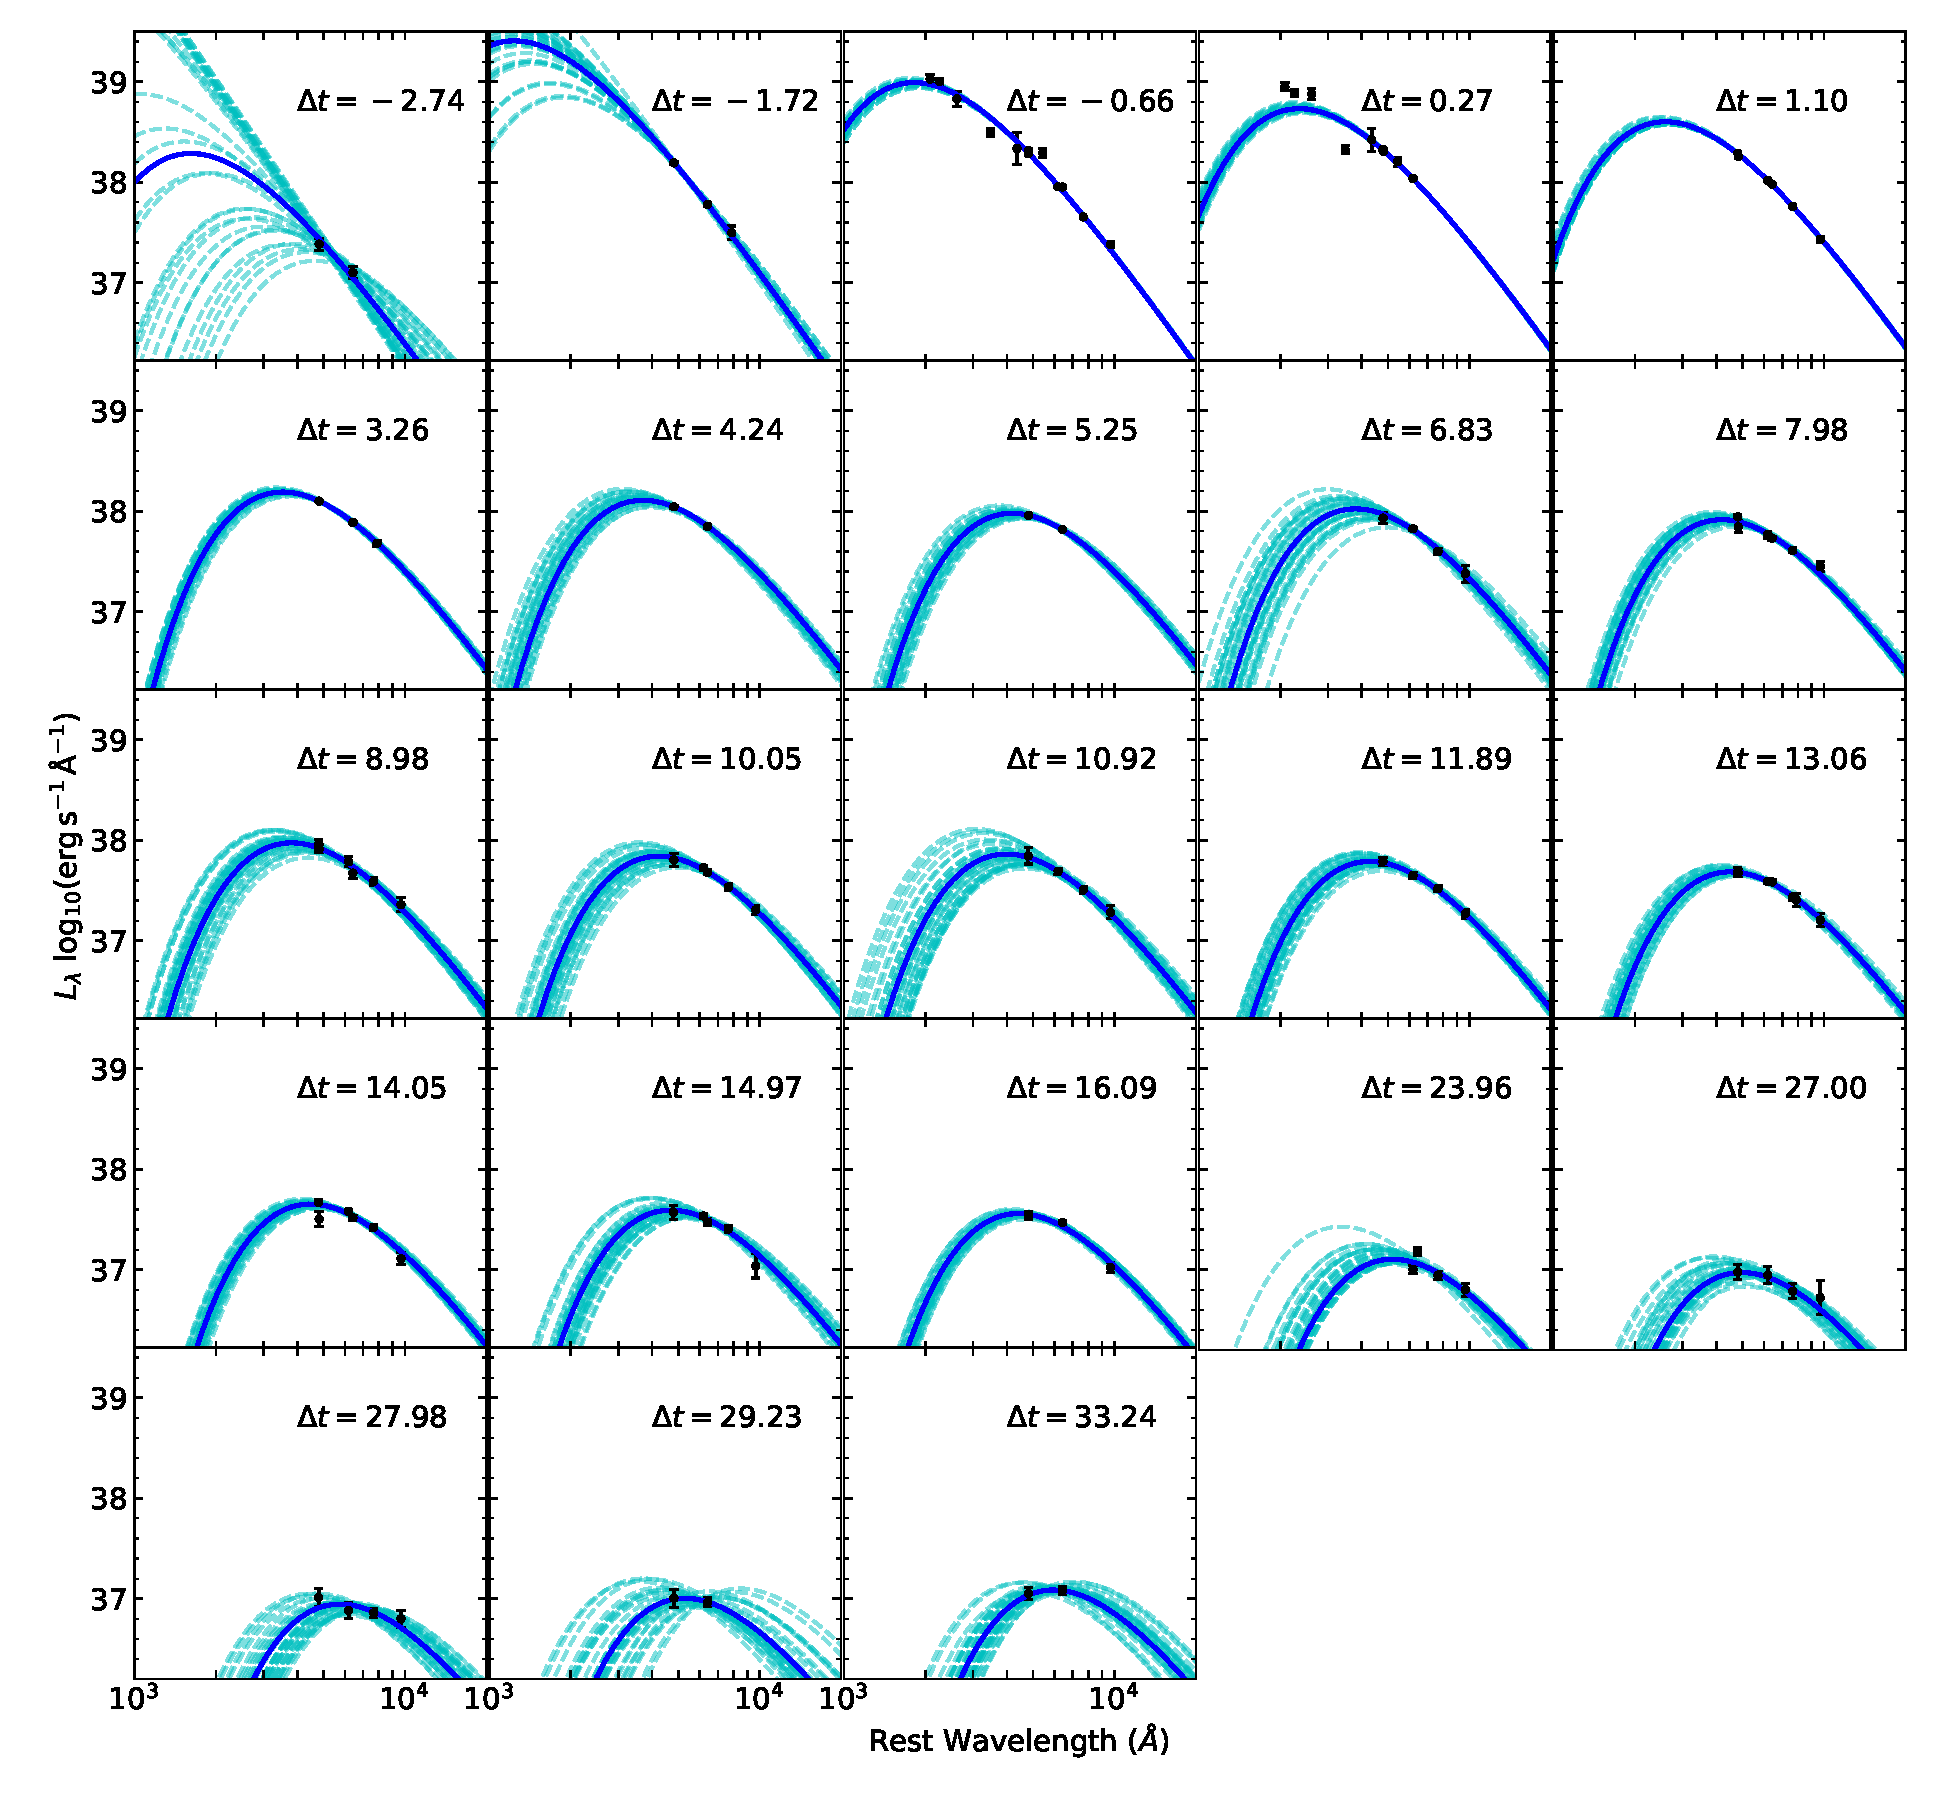
\includegraphics[width = 0.9\textwidth]{figures/seds.pdf}
    \caption{The maximum MCMC a posteriori model fits to $Swift$/UVOT and optical photometry for 
    AT2019dge.  \label{fig:seds}}
\end{figure*}
\begin{table}[!htbp] 
	\centering 
	\caption{Physical evolution of SN2019dge from blackbody fits.} 
	\begin{tabular}{lrrr} 
		\hline 
		$\Delta t$ & $L (10^{41} \,{\rm erg\,s^{-1}})$ & $R$ ($10^{3}\,R_\odot$) & $T$ ($10^3$\,K) \\ 
		\hline
		-2.74 & $2.98^{+578.84}_{-1.41}$ &$1.45^{+1.14}_{-1.14}$ &$14.21^{+101.35}_{-5.12}$  \\
		-1.72 & $44.63^{+43.85}_{-15.84}$ &$2.20^{+0.44}_{-0.46}$ &$22.75^{+7.60}_{-4.14}$  \\
		-0.66 & $27.15^{+1.13}_{-1.07}$ &$3.48^{+0.08}_{-0.08}$ &$15.96^{+0.34}_{-0.33}$  \\
		0.27 & $19.26^{+0.77}_{-0.72}$ &$4.92^{+0.14}_{-0.14}$ &$12.32^{+0.29}_{-0.28}$  \\
		1.10 & $15.72^{+0.46}_{-0.42}$ &$5.39^{+0.14}_{-0.14}$ &$11.20^{+0.23}_{-0.22}$  \\
		3.26 & $8.34^{+0.22}_{-0.20}$ &$7.26^{+0.46}_{-0.44}$ &$8.23^{+0.31}_{-0.28}$  \\
		4.24 & $7.29^{+0.26}_{-0.22}$ &$7.38^{+0.88}_{-0.83}$ &$7.88^{+0.54}_{-0.46}$  \\
		5.25 & $6.10^{+0.16}_{-0.15}$ &$8.77^{+0.78}_{-0.73}$ &$6.92^{+0.33}_{-0.30}$  \\
		6.83 & $6.18^{+0.63}_{-0.46}$ &$7.09^{+1.01}_{-0.92}$ &$7.72^{+0.75}_{-0.62}$  \\
		7.98 & $5.29^{+0.24}_{-0.21}$ &$8.00^{+0.75}_{-0.70}$ &$6.99^{+0.39}_{-0.35}$  \\
		8.98 & $5.49^{+0.44}_{-0.36}$ &$6.79^{+0.94}_{-0.85}$ &$7.66^{+0.65}_{-0.56}$  \\
		10.05 & $4.55^{+0.37}_{-0.27}$ &$7.42^{+1.03}_{-0.96}$ &$6.99^{+0.63}_{-0.52}$  \\
		10.92 & $4.49^{+0.64}_{-0.44}$ &$6.63^{+1.25}_{-1.06}$ &$7.37^{+0.93}_{-0.75}$  \\
		11.89 & $4.04^{+0.24}_{-0.21}$ &$7.42^{+0.83}_{-0.75}$ &$6.79^{+0.45}_{-0.40}$  \\
		13.06 & $3.34^{+0.10}_{-0.10}$ &$7.52^{+0.69}_{-0.66}$ &$6.43^{+0.32}_{-0.29}$  \\
		14.05 & $3.08^{+0.10}_{-0.09}$ &$7.05^{+0.63}_{-0.59}$ &$6.51^{+0.32}_{-0.29}$  \\
		14.97 & $2.82^{+0.15}_{-0.12}$ &$7.30^{+1.21}_{-1.06}$ &$6.25^{+0.57}_{-0.49}$  \\
		16.09 & $2.45^{+0.09}_{-0.09}$ &$6.17^{+0.59}_{-0.58}$ &$6.56^{+0.33}_{-0.29}$  \\
		23.96 & $1.02^{+0.07}_{-0.06}$ &$5.47^{+1.23}_{-1.12}$ &$5.59^{+0.74}_{-0.54}$  \\
		27.00 & $0.72^{+0.08}_{-0.08}$ &$4.08^{+1.26}_{-1.01}$ &$5.93^{+0.91}_{-0.70}$  \\
		27.98 & $0.78^{+0.07}_{-0.06}$ &$5.73^{+1.68}_{-1.29}$ &$5.10^{+0.68}_{-0.57}$  \\
		29.23 & $0.83^{+0.11}_{-0.09}$ &$4.76^{+2.47}_{-1.56}$ &$5.64^{+1.23}_{-0.93}$  \\
		33.24 & $1.09^{+0.16}_{-0.11}$ &$6.99^{+2.47}_{-1.74}$ &$5.02^{+0.65}_{-0.56}$  \\
		\hline 
	\end{tabular} 
	\label{tab:bbfit} 
\end{table} 


\subsection{Modelling Early Light Curve} \label{subsec:p15fit}
\begin{deluxetable}{llc}[htpb!]
	\tablecaption{Shock cooling model parameters $\theta$ and their priors \label{tab:P15priors}}
	\tablehead{
		\colhead{$\theta$}
		& \colhead{Description}
		&\colhead{Prior}
	}
	\startdata
	${\rm log}R_{\rm ext}$ & log$_{10}$ of extented material radius in cm  & 
	$\mathcal{U}(-5, 25)$ \\
	${\rm log}M_{\rm ext}$ &  log$_{10}$ of extented material mass in $M_\odot$  & $\mathcal{U}(-4, 
	0)$\\
	$t_\mathrm{exp}$ & explosion epoch in MJD relative to $58583.2$& $\mathcal{U}(-8,-2.76)$ \\
	$E_{51}$ & SN energy divided by $10^{51}\,{\rm erg}$ & $\mathcal{U}(0.01, 10)$ \\
	$E_{\rm ext, 49}$ & $E_{\rm ext}$ divided by $10^{49}\,{\rm erg}$ & 
	$\mathcal{U}(0.1,100)$ \\
	\enddata
\end{deluxetable}



\begin{figure}[htbp!]
	\centering
	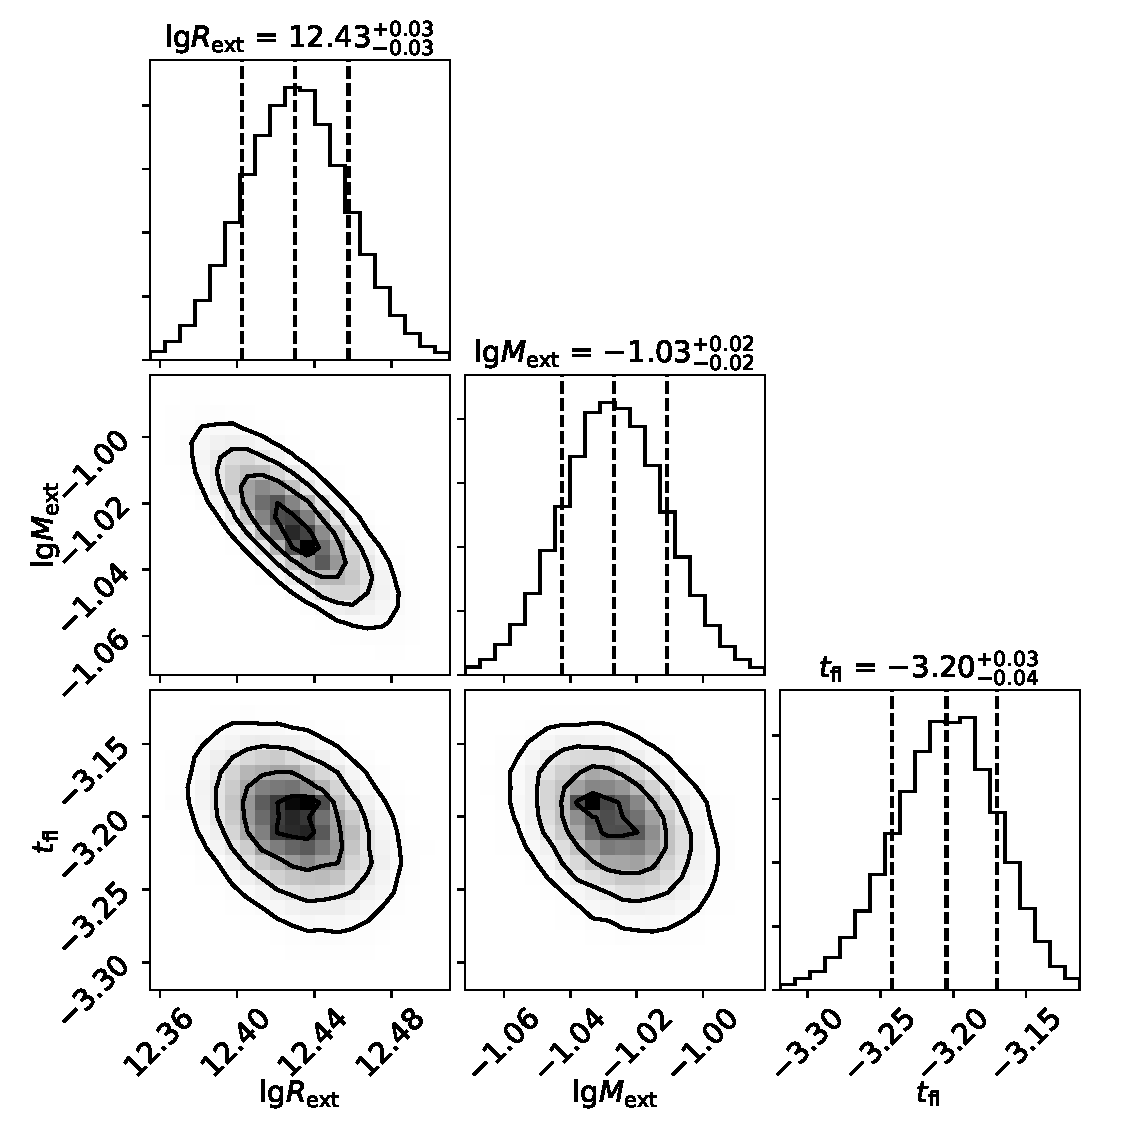
\includegraphics[width=\columnwidth]{figures/corner_P15.pdf}
	\caption{Corner plot showing the posterior constraints on ${\rm lg}R_{\rm ext}$, ${\rm lg}M_{\rm 
			ext}$, and $t_\mathrm{fl}$. Marginalized one-dimensional distributions are shown along the 
		diagonal, along with the median estimate and the 68\% credible region (shown with vertical 
		dashed 
		lines).	\label{fig:pirocorner}}
\end{figure}
To model the early light curve with the P15 model, we fix $\kappa\sim0.2\,{\rm cm^2\, g^{-1}}$ as 
appropriate for a hydrogen-deficient ionized gas, and assign wide flat priors for all model parameters, 
as summarized in Table~\ref{tab:P15priors}. We only include observations up to $\Delta t = 2$\,d in 
the fitting. We found that this particular choice of $\Delta t$ --- 2\,d instead of 1\,d or 3\,d --- in 
general does not affect the final inference for the model parameters. Figure~\ref{fig:pirocorner} shows 
the corner plot of ${\rm lg}R_{\rm ext}$, ${\rm lg}M_{\rm 	ext}$, and $t_\mathrm{fl}$. For clarity, 
$E_{51}$ and $M_{\rm core}$ are excluded as they do not exhibit strong covariance with the 
parameters shown here. These two parameters are highly anti-correlated with each other over a wide 
range of their priors. We find $E_{51}\propto M_{\rm core}^{0.7}$, as implied by 
\citet[][Eq~3]{Piro2015}. The amount of energy passed into the extended material is well constrained to 
be $E_{\rm ext} = (1.15\pm 0.07) \times 10^{50}\,{\rm erg\, s^{-1}}$.

\begin{figure}[htbp!]
	\centering
	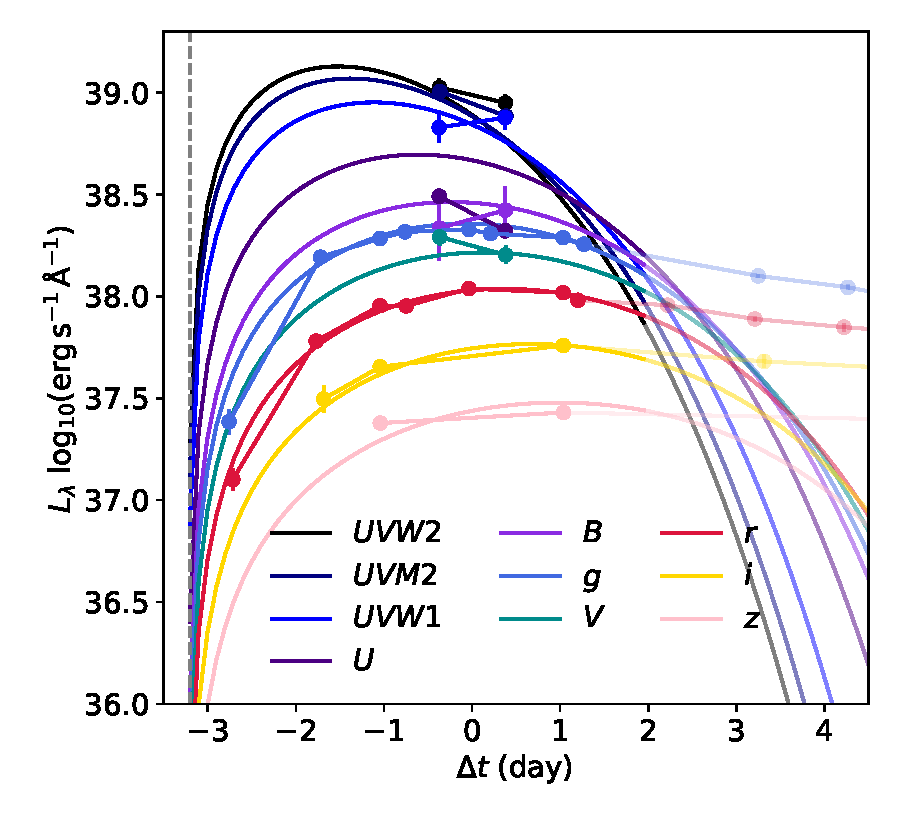
\includegraphics[width=\columnwidth]{figures/P15model.pdf}
	\caption{Cooling emission model fit to the early light curve of AT2019dge. 
		Data excluded from the fitting are shown as transparent circles. 
		The maximum a posteriori model is shown via solid lines.
		The vertical dashed line shows the median 1-D marginalized posterior value of
		$t_{\rm fl}$.
		\label{fig:piromodel}}
\end{figure}

The maximum a posteriori model is visualized by solid lines in Figure~\ref{fig:piromodel} color-coded in 
different filters. Note that the fitting is not perfect at the UV bands since 
the SED is not exactly a blackbody at peak (see Figure~\ref{fig:seds}). The rising part of the model 
does not closely match to data due to the ignorance of the density structure of the stellar profile. 
Nevertheless, the peak of the light curve is well captured by this model.

\subsection{Modelling the Main Peak}\label{subsec:arnettfit}

For $^{56}\rm Ni \rightarrow ^{56}Co \rightarrow ^{56}Fe$ decay powered explosions, the energy 
deposition rate is
\begin{align}
\varepsilon_{\rm rad} =&\varepsilon_{\rm Ni, \gamma} (t) + \varepsilon_{\rm Co, \gamma} (t) 
\label{eq:heatTotal} \\
\varepsilon_{\rm Ni, \gamma} (t)   =& \epsilon_{\rm Ni}e^{-t/\tau_{\rm Ni}}  \label{eq:heatNi}\\
\varepsilon_{\rm Co, \gamma} (t)   =& \epsilon_{\rm Co} \left( e^{-t/\tau_{\rm Co}} - e^{-t/\tau_{\rm 
			Ni}} \right) \label{eq:heatCo}
\end{align}
where $\epsilon_{\rm Ni}= 3.90 \times 10^{10} \, {\rm erg\,g^{-1}\,s^{-1}}$, $\epsilon_{\rm Co}=6.78\times 
10^{9} \, {\rm erg\,g^{-1}\,s^{-1}}$, $\tau_{\rm Ni}=8.8$\,d and $\tau_{\rm Co}=111.3$\,d are the decay 
lifetimes of $^{56}\rm Ni$ 
and $^{56}\rm Co$ \citep{Nadyozhin1994}. The effective heating rate is modified by the probability of 
thermalization, and thus $\varepsilon_{\rm heat} \leq \varepsilon_{\rm rad}$.

The bolometric light curve can be generally divided into the 
photospheric phase and the nebula phase. The photospheric phase can be modelled using Equations 
given in \citet[][Appendix A]{Valenti2008}, with modifications given 
by \citet[][Eq.~3]{Lyman2016}, 
\begin{align}
 L_{\rm phot} (t) =& M_{\rm Ni} {\rm e}^{-x^2} \times \notag  \\
 & \Big[ (\epsilon_{\rm Ni} - \epsilon_{\rm Co}) \int_0^x (2z {\rm e}^{-2zy+z^2}){\rm d} z \notag \\
 & + \epsilon_{\rm Co} \int_0^x (2z {\rm e}^{-2zy+2zs + z^2}) {\rm d} z \Big]
\end{align}
where $x = t/\tau_{\rm m}$, $y = \tau_{\rm m} / (2\tau_{\rm Ni})$,
\begin{align}
s &= \frac{\tau_{\rm m} (\tau_{\rm Co} - \tau_{\rm Ni})}{2 \tau_{\rm Co} \tau_{\rm Ni}}, \notag \\
\tau_{\rm m} &= \left( \frac{2\kappa_{\rm opt} M_{\rm ej}}{13.8 c v_{\rm phot}}\right)^{1/2}  
\label{eq:taum}
\end{align}

At the nebula phase the SN ejecta becomes optically thin, such that the delay between the energy 
deposition from radioactivity and the optical radiation becomes shorter. The bolometric luminosity is 
then equal to 
the rate of energy deposition: $L_{\rm neb}(t) = Q(t)$. At any given time, the energy deposition rate 
$Q(t)$ is \citep{Wheeler2015, Wygoda2019}:
\begin{align}
Q(t) \approx Q_{\gamma}(t) \left( 1 - e^{-(t_0/t)^2}\right) % Q_{\rm pos}(t),
\end{align}
where $Q_{\gamma}(t) = M_{\rm Ni}\varepsilon_{\rm rad}$ is the energy release rate of gamma-rays,
$t_0$ is the time at which the ejecta becomes optically thin to gamma rays. Here the difference 
between energy deposition rate of gamma-rays and positrons  is neglected.
%\begin{align}
%Q_{\rm pos}(t) &= M_{\rm Ni}\varepsilon_{\rm Co, pos}(t)\\
%\varepsilon_{\rm Co, pos}(t) &=  2.3\times 10^{8} \left( e^{-t/t_{s, {\rm Co}}} - e^{-t/t_{s, {\rm Ni}}}\right)
%\end{align}

\begin{deluxetable}{llc}[htpb!]
	\tablecaption{$^{56}$Ni decay model parameters $\theta$ and their priors \label{tab:Nidecaypriors}}
	\tablehead{
		\colhead{$\theta$}
		& \colhead{Description}
		&\colhead{Prior}
	}
	\startdata
	$\tau_{\rm m}$ &characteristic photon diffusion time in day  & $\mathcal{U}(1, 20)$ \\
	${\rm log}M_{\rm Ni}$ &  log$_{10}$ of nickel mass in $M_\odot$  & $\mathcal{U}(-4, 0)$\\
	$t_0$ & characteristic $\gamma$-ray escape time in day & $\mathcal{U}(20,  100)$  \\
	\enddata
\end{deluxetable}

\begin{figure}[htbp!]
	\centering
	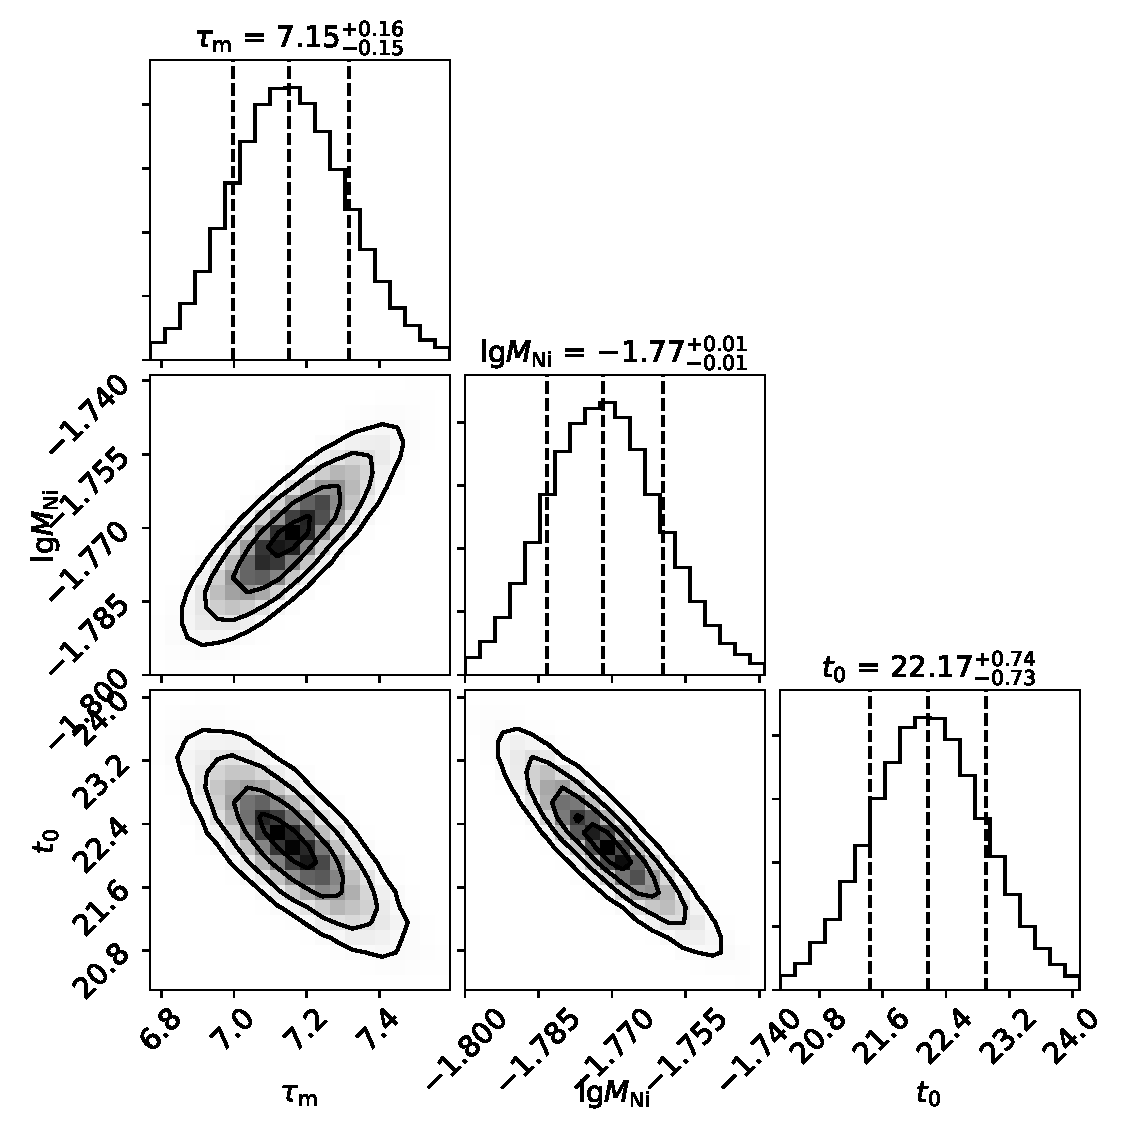
\includegraphics[width=\columnwidth]{figures/corner_arnett_modified.pdf}
	\caption{Corner plot showing the posterior constraints on $\tau_{\rm m}$, ${\rm lg}M_{\rm 
			Ni}$, and $t_0$. Marginalized one-dimensional distributions are shown along the 
		diagonal, along with the median estimate and the 68\% credible region (shown with vertical 
		dashed 
		lines).	\label{fig:Nidecaycorner}}
\end{figure}

To fit the shock cooling subtracted bolometric light curve with a simple radioactive decay model, we do 
not divide the data into photosperic phase and nebula phase, but instead adopt the following formula 
for the whole light curve:
\begin{align}
	L(t) = L_{\rm phot}(t)  \left( 1 - e^{-(t_0/t)^2}\right) 
\end{align}
Priors or the model parameters are summarized in Table~\ref{tab:Nidecaypriors}, and Figure 
\ref{fig:Nidecaycorner} shows the coner plot of $\tau_{\rm m}$, lg$M_{\rm Ni}$, and $t_0$.

\section{UV and Optical Spectroscopy} \label{sec:appspec}
\subsection{Data} \label{subsec:appspec_data}
The log of UV and optical spectroscopy is presented in Table \ref{tab:spec}.

\begin{table*}
	\caption{Log of AT2019dge spectroscopy. \label{tab:spec}}
	\centering
	\begin{tabular}{llrccc}
	\toprule
	Start Time  & Instrument & $\Delta t$& Exposure Time & Airmass & Resolution\\
	(UTC) & & (day)& & (s)& (FWHM $\AA$)\\
	\midrule
	% # DATE-OBS= '2019-04-09T03:30:28.157'             % # UTSTART = '03:30:28.157'
	% # MJD     =         58582.146159
	2019 Apr 09 03:30:28 & LT+SPART  & $-1.1$&  500   & 1.800 & 18 \\
	% # DATE-OBS= '2019-04-10T03:06:09.604'
	% # UTSTART = '03:06:09.604'
	% # MJD     =         58583.129278
	2019 Apr 10 03:06:10 & LT+SPART & $-0.1$ &  500   & 1.800 & 18 \\
	% LRIS
	2019 Apr 10 14:21:44 & Keck1+LRIS & $+0.4$ & 300 & 1.169 & 6 \\
	% HST
	2019 Apr 12 05:08:00 & HST+WFC3+UVIS & $+12.0$& 2$\times$250 & --- & 43\\
	% DBSP
	2019 Apr 24 11:06:43 & P200+DBSP & $+14.3$& 1200 & 1.047 & 3--5\\
	% LRIS
	2019 Jul 04 11:49:18   & Keck1+LRIS & $+85.3$& 1740 & 1.421 & 6\\
	% LRIS
	2019 Aug 31 08:04:58   & Keck1+LRIS &$+143.1$ & 1150 & 1.409 & 6  \\
	% LRIS
	2019 Sep 28 08:14:27   & Keck1+LRIS & $+171.1$& 600 & 2.165 & 6\\
	% LRIS
	2020 Feb 18 15:23:40   & Keck1+LRIS & $+314.4$& 1450 & 1.384 & 6\\
	\bottomrule
\end{tabular}
\end{table*}

%The final spectrum taken was a LRIS spectrum from $+111?$\,days which showed narrow nebular 
%emission lines from the host galaxy but no detectable flux from AT2019dge. 
We use line centers of nebular lines to derive the spectroscopic redshift of the host (Table 
\ref{tab:eml_host}). The mean of all centroids gives $z = 0.0213 \pm 0.0001$.

\begin{table}[htbp!]
	\caption{Line fluxes from the host galaxy of AT2019dge extracted from the Keck/LRIS spectrum 
	obtained on Aug xx 2019. }\label{tab:eml_host}
	\centering
	\begin{tabular}{llcc}
		\toprule
		Transition			& $\lambda_{\rm obs}$& $F$	\\
		& (\AA)	& $\left(10^{-16}~{\rm erg\,cm}^{-2}\,{\rm s}^{-1}\right) $ \\
		\midrule
		%{[\ion{O}{2}]}$\lambda\lambda$3726,3729 &$ 3848.17 \pm 0.05	$&$	334.5	\pm	6.23	$\\
		%{[\ion{Ne}{3}]}$\lambda$3869			& $ 3993.50 \pm 0.16	$&$	82.34	\pm	6.18	$\\
		%\ion{He}{1}$\lambda$3889,H-8			& $ 4014.49 \pm 0.16	$&$	29.01	\pm	4.73	$\\
		%{[\ion{Ne}{3}]}$\lambda$3968,H$\epsilon$& $ 4096.66 \pm 0.26	$&$	36.61	\pm	3.98	$\\
		%H$\delta$ 								& $ 4233.87 \pm 0.13	$&$	44.88	\pm	2.59	$\\
		%H$\gamma$								& $ 4480.20 \pm 0.10	$&$	81.95	\pm	3.74	$\\
		%{[\ion{O}{3}]}$\lambda$4364 			& $ 4503.68 \pm 0.10	$&$	15.01	\pm	2.69	$\\
		H$\beta$								& $ 4862.35 \pm 0.21	$ &$	32.45 \pm 2.08		$\\%yes
		%{[\ion{O}{3}]}$\lambda$4960 			& $ 5118.61 \pm 0.04	$&$	352.42	\pm	6.50	$\\
		{[\ion{O}{III}]}$\lambda$5007				& $5007.06 \pm 0.55$ &$67.56 \pm 13.52	$\\%yes
		%\ion{He}{1}$\lambda$5877				& $ 6064.21 \pm 0.20	$&$	27.04	\pm	2.30	$\\
		%\ion{O}{1}$\lambda$6302				& $ 6502.18 \pm 1.08	$&$	6.72	\pm	2.94	$\\
		%{[\ion{N}{2}]}$\lambda$6549				& $ 6758.16 \pm 0.02	$&$	11.15	\pm	6.73	$\\
		H$\alpha$								&$6562.07 	\pm 0.03$   & $115.79 \pm 1.16	$\\%yes
		{[\ion{N}{II}]}$\lambda$6583				& $6582.62 \pm 0.08$ &$	8.89 \pm 0.37	$\\%yes
		%{[\ion{He}{1}]}$\lambda$6678			& $ 6890.29 \pm 0.14	$&$	7.88	\pm	2.19	$\\
		%{[\ion{S}{2}]}$\lambda$6718 			& $ 6931.83 \pm 0.10	$&$	41.76	\pm	2.38	$\\
		%{[\ion{S}{2}]}$\lambda$6732 			& $ 6946.68 \pm 0.10	$&$	28.15	\pm	2.19	$\\
		\bottomrule
	\end{tabular}
	\tablecomments{All measurements are corrected for Galactic reddening.}
\end{table}

\begin{table}
	\centering
	\caption{Photometry of the host galaxy}\label{tab:host_phot}
	\begin{tabular}{ccc}
		\toprule
		Instrument/	    & $\lambda_{\rm eff}$   & Brightness		\\
		Filter          & (\AA)                 & (mag)             \\
		\midrule
		SDSS/$u'$ 		& 3594.9  & $ 19.336	 \pm 0.039$	\\
		SDSS/$g'$ 		& 4640.4  & $ 18.322 \pm 0.009$	\\
		SDSS/$r'$ 		& 6122.3  & $ 17.913	 \pm 0.009 $	 \\
		SDSS/$i'$ 		& 7439.5     &$ 17.745  \pm 0.010$\\
		SDSS/$z'$ 		& 8897.1     &$ 17.580 \pm 0.031$\\
		WISE/$W1$ 		& 33526.0    &$ 15.938 \pm 0.037$\\
		WISE/$W2$   & 46028.0    &$ 15.982 \pm  0.082$\\
		\bottomrule
	\end{tabular}
	\tablecomments{SDSS \citep{Alam2015} measurements are reported in the AB system. AllWISE 
	\citep{Cutri2013} measurements are in the Vega system and the conversion to flux density are 
	performed using \citet[][Table~1]{Jarrett2011}. Values 
	are not corrected for reddening. }
\end{table}
% no record in URAT1
% no record in GALEX
\subsection{Mass Loss Estimate from \ion{He}{II}} \label{subsec:flash}
Assuming that the CSM around the progenitor has a sperical wind-density profile of the form
$\rho = K r^{-2}$, where $r$ is distance from the progenitor, $K\equiv \dot M / (4\pi v_{\rm w})$ is the 
mass loading parameter, $v_{\rm w}$ is the wind/outburst velocity, and $\dot M$ is the mass loss rate. 
The integrated mass of the emitting material from $r$ to $r_1$ is 
\begin{align}
 M_{\rm He} = \int_{r}^{r_1}4\pi r^2 \rho(r) {\rm d}r4\pi K(r_1 - r) = 4\pi K \beta r
\end{align}
where $\beta \equiv (r_1 - r) /r $ is assumed to be of the order unity.

Following \citet{De2018}, we can relate the mass of the \ion{He}{II} region to the \ion{He}{II} 
$\lambda4686$ line luminosity using 
\begin{align}
	L_{\lambda 4686} \approx \frac{A n_e M_{\rm He}}{m_{\rm He}} \label{eq:L4686}.
\end{align}
Here
\begin{align}
	A = \frac{4\pi j_{\lambda 4686}}{n_e n_{\rm He^{++}}},
\end{align}
$ j_{\lambda4868}$ (in ${\rm erg \, cm^{-3}\, s^{-1}\, sr^{-1}}$) is the emission coefficient for the 
$\lambda4686$ transition. $m_{\rm He}$ is mass of a He nucleus, $n_{\rm He^{++}}$ is the number 
density of doubly ionized helium and $n_e$ is the number density of electrons.

Assuming a temperature of $10^4$\,K, electron density of $10^{10}\,{\rm cm^{-3}}$, and Case B 
recombination, we get $A=1.32\times 10^{-24}\,{\rm erg\, cm^{3}\, s^{-1}}$ \citep{Storey1995}. 
Assuming $n_e = 2 n_{\rm He^{++}}$ and using the density profile, Eq.~(\ref{eq:L4686}) can be written 
as
\begin{align}
	L_{\lambda 4686} \approx \frac{8\pi A \beta}{m_{\rm He}^2} \frac{K^2}{r}.
\end{align}

The location of the emitting region can be constrained by requiring that the Thompson optical depth 
($\tau$) in the region must be small for the lines to escape. We require
\begin{align}
 \tau &= n_e \sigma_{\rm T} \int_{r}^{r_1} {\rm d}r = 2n_{\rm He^{++}} \sigma_{\rm T} r\beta = 
 \frac{2\sigma_{\rm T}r\beta}{m_{\rm He}} 
 \frac{K}{r^2} \notag \\
 & = \frac{2\sigma_{\rm T}K\beta}{m_{\rm He}r} \lesssim 1
\end{align}
Thus
\begin{align}
 r^2 &\gtrsim  \left (\frac{2\sigma_{\rm T}\beta}{m_{\rm He}} \right)^2 \frac{L_{\lambda 4686} m_{\rm 
 He}^2 r }{8\pi A \beta } \notag \\
 r & \gtrsim L_{\lambda 4686} \frac{\sigma_{\rm T}^2  \beta }{2\pi A }
\end{align}

The $+0.4$\,d emission line flux is meausred to be $F = (8.37\pm 0.65)\times10^{-16}\,{\rm erg\, 
cm^{-2}\,s^{-1}}$, correslonding to $L_{\lambda 4686} = 8.6\times 10^{38}\,{\rm erg\, s^{-1}}$. Hence, 
we get $r \gtrsim 4.8 \times 10^{13} \beta \,{\rm cm}$, $K \gtrsim 1.2\times 10^{14} \, {\rm 
g\,cm^{-1}}$, and $M_{\rm He} \gtrsim 3.6\times 10^{-5} \beta^2\, M_{\odot}$.


Note that the above calculate only assumes that recombination is the primary line-emitting mechanism, 
and that collisional excitation and de-excitation processes can be ignored. \todo{rewrite this: the 
inferred radius ot optically thin material is larger than the envelope producing the early shock cooling 
emission as seen inthe light curve, and suggests that the highly ionized lines likely arise from a lower 
density extension of the same envelope?}

\todo{Ask Kishalay: what is the light travel time blah blah argument -- Now that the recombination 
timesclae is very short, }

\bibliography{at2019dge}{}
\bibliographystyle{aasjournal}

\end{CJK*}


\end{document}